\graphicspath{{appendices/}{regional_mosaics/}{Figures/}}
% \graphicspath{{Figures/}}

\chapter[LineaMapper on Galileo RegMaps]{Length, width, and relative age analysis of lineaments in the Galileo regional maps with LineaMapper}
\label{chapter:regional_mosaics}

\sidechaptersummary{Adapter for large segmentation models, supervised segmentation performance improvement, applications to domain generalization}
% \desctotoc{Test1 --- Test 2}

\subsubsection{Synopsis}The Solid-State Imaging (SSI) system on board the Galileo spacecraft returned two north-south image mosaics covering swaths of the trailing and leading hemispheres of Europa at a regional scale (\qty{215}{\m~\px^{-1}}). These regional mosaics (``RegMaps'') are of great value as they show Europa’s extensive regional-scale tectonic features almost from pole to pole and were acquired under similar illumination conditions. A complete lineament map of the RegMaps has not yet been accomplished, although a lineament study could constrain resurfacing events and formation mechanisms.

We aim to gain statistical insights into lineament distributions and characteristics of length, width, and relative age, which we assess by the number of fragmentations per kilometer in different geological terrains contained within the RegMaps. We find evidence that only the latest formed linear features remain discernible following the disruption by chaos terrain. Because mapping of lineaments is time-intensive and subjective, especially in noisy images of densely ridged regions on Europa, we employ the deep-learning tool LineaMapper to make mapping faster and more consistent over large areas. Guided by LineaMapper, we produce a validated lineament map of the southern leading hemisphere part of the RegMaps. % Furthermore, a new version of LineaMapper makes mapping faster and more consistent over large areas, 
The manually revised map is utilized as additional training data of 2140 lineaments, with which we train LineaMapper v1.1 and v2.0, using two different deep learning models. 
Based on this map, we find a lineament density of 15\% in chaos and 65\% in ridged plains, which we use to fully-automatically classify units of chaos and ridged plains in the full RegMaps. We find good agreement with a global geologic map.

We conclude that LineaMapper can be employed for an objective assessment of Europa's previously unresolved regions with the Europa Imaging System on Europa Clipper. Finally, we make the full output of LineaMapper available and offer an interactive tool for testing LineaMapper v2.0, which utilizes the Segment Anything model by Meta.

\subsubsection{Publication}This appendix chapter is based on a publication that is under review, and its contents have been modified slightly to be more consistent with the rest of the thesis. More specifically, the style of \Cref{fig_count_normalised,fig_17ESREG02_area_density} has been adapted. Moreover, in order to alleviate the space, Section 3 of the original publication containing the summary has been left out, as well as the supplementary material.

\subsubsection{Author contributions}Most of the work for this publication has been done by Caroline Haslebacher. The contributing authors were Louise M. Prockter, Erin J. Leonard, Alyssa R. Rhoden, and Nicolas Thomas. My contribution consisted of implementing and training the SAM model on the regional mosaics.

\section{Introduction} \label{sec:intro}
%\subsection{Linear surface features on Europa}
% introduce bands, rc, db, ul here?

Different forms of lineaments may evolve out of initial cracks in the icy surface of Jupiter’s moon Europa\sidecite{Figueredo2004, Bradak2023b, Greenberg1998, ProckterPatterson2009}. Therefore, all types of lineaments have the potential to link to subsurface liquid water, as evidence is found for Enceladus\sidecite{Hansen2006, Sladkova2021, Ingersoll2016}. This makes lineaments of high interest to Europa's potential as a habitable world\sidecite{Daubar2024}.

\plainwidefig{1}{regional_mosaics/Figures/basemap_excerpt.png}{Global map with regional maps (RegMaps) in shades of red and the region for the manually revised lineament map (red box). Top: Basemap from USGS~\cite{USGS2002}. Bottom: Global geologic map~\cite{Leonard2024}.}{fig:RegMaps_basemap}

The Solid State Imager (SSI) onboard NASA’s Galileo spacecraft mapped approximately 10\% of Europa’s surface at a regional resolution of 200-230 m/px. Two north-south covering image mosaic swaths acquired under similar illumination conditions portray parts of the leading and trailing hemispheres (in the following abbreviated as ``RegMaps'', see \Cref{fig:RegMaps_basemap}). Because of the north-south extent and leading/trailing locations, these image mosaics enable the study of regional geological processes across a range of latitudes and longitudes\sidecite{Figueredo2003, Sarid2004, Patterson2006, Collins2022}. However, they do not enable features to be linked globally. 
Unfortunately, the most complete existing geologic maps\sidecite{Figueredo2004} of the RegMaps are not available in a digitised version. Furthermore, the level of detail with respect to the mapped lineaments is insufficient for an extensive lineament analysis due to the scale of the map. The map we present in this work is at a larger scale and therefore reveals fine lineae in areas previously mapped as ``ridged plains''\sidecite{Greeley2000}.

\plainwidefig{1}{regional_mosaics/Figures/Features_examples_grid.png}{A selection of Europan surface type features.}{fig:features_exs}

The surface of Europa is characterised by tectonic features overlaid by a small number of impact craters and disrupted in some regions by chaos terrain. Regional and global mapping has identified three broad episodes of deformation\sidecite{Prockter1999, Figueredo2000, DoggettEuropaBook2009, Leonard2024}. The oldest identifiable tectonic unit, ridged plains (\Cref{fig:features_exs}.A), is widespread across the surface. Characterised by multidirectional, mostly high-albedo linear ridges, the ridged plains unit overlaid by all later structures such that it appears as background plains material\sidecite{Daubar2024, Leonard2024}. Next in the stratigraphic sequence are bands, linear or curvilinear dilational features that have formed by symmetrical spreading from a crack or double ridge with new subsurface material filling the gap\sidecite{Greeley2000, Tufts2000}, analogous to mid-ocean ridges on Earth\sidecite{Sullivan1998} (\Cref{fig:features_exs}.B). Band morphologies fall into two major types: relatively smooth material comprised of small hummocks, and more rugged subparallel ridges\sidecite{Prockter2002}, that may be related to the band’s opening rate\sidecite{Stempel2005}. The youngest episode of deformation is the result of ``chaos'' formation, in which the surface has been disrupted from below, resulting in the breakup of preexisting terrain into discontinuous blocks of icy material set into a darker, hummocky matrix (\Cref{fig:features_exs}.C)\sidecite{Greeley2000}. Microchaos consists of smaller, discontinuous subcircular patches of chaos\sidecite{Pappalardo1998, Spaun2002, Noviello2019}, whose relationship to the larger chaos regions is not yet understood\sidecite{Collins2009}. Chaos may result from upwelling diapirs of thermally or compositionally buoyant material intersecting the surface\sidecite{Greenberg1999, Sotin2002, Figueredo2002, Schmidt2011, Collins2009} and it has been proposed that a periodic thinning and thickening of the ice shell drives periodic formation of chaos and regional plains terrain on a timescale comparable with the inferred surface age of 20 to 200 Myrs\sidecite{Bierhaus2009, Hussmann2004}. The regional plains unit makes up for 53\% of the global coverage, which makes it the most common unit, followed by chaos terrain with 40\%\sidecite{Leonard2024}. 

One feature that has formed throughout Europa’s stratigraphic history is the double ridge, which is widespread across the surface\sidecite{Figueredo2000}. Consisting of a distinct V-shaped trough flanked on each side by a single ridge\sidecite{Head1999, Greeley2000} (\Cref{fig:features_exs}.D), double ridges are observed at a range of size scales and as linear or curvilinear features a few tens of meters to hemispherical in length, and some forms appear related to diurnal tides\sidecite{Hoppa1999a}. Multiple models have been proposed for their formation, however, none are able to fully match all the observations\sidecite{ProckterPatterson2009, Daubar2024}. Ridge complexes are less common and consist of several adjacent parallel or anastomosing sets of double ridges\sidecite{Greeley2000} (\Cref{fig:features_exs}.E). Their formation mechanisms remain obscure\sidecite{Kattenhorn2009}. The youngest tectonic features on Europa are troughs, which appear similar to the V-shaped troughs of double ridges but lack the flanking ridges\sidecite{Greeley2000} (\Cref{fig:features_exs}.F). These are not observed in older terrains, perhaps because they fade and are overlooked easily\sidecite{Greeley2000}, but it is likely that they have been exploited to form other types of tectonic features\sidecite{Kattenhorn2009}. 
 
Because so little is known about how Europa’s tectonic features relate to the stresses that form them, including diurnal, non-synchronous, and polar wander\sidecite{Kattenhorn2009, Sotin2009}, the extent to which the tectonic landforms penetrate the ice shell is not well understood. Knowledge of the pathways that these features create or exploit is critical to understanding how material moves through the ice shell, and whether liquid water, including the ocean, is accessed. 
% End of Louise's paragraph

A global geologic map\sidenote{Such as the one in~\cite{Leonard2024}, or \Cref{fig:RegMaps_basemap}}, provides the global context for current missions to Europa, namely JUICE and Europa Clipper. The Europa Imaging System (EIS) on NASA's Europa Clipper will deliver a global view of Europa at a resolution $\leq$100 m/px in the 2030's\sidecite{TurtleSSR}. This global dataset will be valuable for lineament cross-cutting analyses and can, for the first time, result in a relative dating of globally interlinked regions\sidecite{Daubar2024}. The relative ages can be compared with absolute age results from crater counting\sidecite{Daubar2024}. Already for this reason alone, a global lineament map is valuable. Furthermore, spatially varying lineament characteristics, for example a regionally varying width of lineaments or different categorical distributions can be used to interpret the geological evolution of Europa's surface.

However, at 100~m/px, lineaments in background ridged plains appear as a dense network, which makes a complete lineament mapping time-consuming. This is where deep learning algorithms can help. \sidecite{Haslebacher2024a} have shown that an automated mapping framework with human validation reduces the workload while still accurately mapping 30-50~\% of lineaments. They trained a regional convolutional neural network, or Mask R-CNN\sidecite{He2018} for lineament mapping in Galileo images showing Europa's surface. Although the time used for mapping can be reduced with LineaMapper v1.0, the tool is not optimised for the resolution and illumination conditions of the RegMaps and would benefit from a larger training dataset. 
To maximise scientific return and flexibility in planning with EIS, an early preparation based on existing imagery is needed to ensure that the evaluation and analysis of all images is optimal. For this, we aim to improve LineaMapper's ability to correctly detect and segment a higher number of lineaments and to provide more continuous segmentation masks.

\plainwidefig[t]{1}{regional_mosaics/Figures/2024_07_17_apply_LineaMapper_scheme_optimised-01.png}{Workflow for assembling LineaMapper's predictions. A moving window tiling algorithm ensures overlapping areas for stitching the predictions together, which are based on smaller tiles of a context image. The need for such an algorithm is especially high for lineaments, which oftentimes run over an area larger than the tile size.}{fig:graphic_Stitching_algo}

Here, we attempt to map all identifiable lineaments in the Galileo RegMaps for an analysis of the evolution of lineament characteristics throughout their formation. This includes lineaments in the ridged plains, which have not frequently been mapped previously, but if mapped, a stratigraphy of lineaments inside ridged plains is insightful\sidecite{Bradak2023}.
To achieve this, we use a new methodology: We use the automated mapping tool LineaMapper\sidecite{Haslebacher2024a} together with a dedicated stitching algorithm to guide the mapping of the RegMaps iteratively. With 2140 new lineaments from a revised part of the RegMaps\sidenote{See red box in \Cref{fig:RegMaps_basemap}}, we train and release LineaMapper v1.1 and v2.0, which are optimised for the RegMaps. Subsequently, the complete Galileo RegMaps are fed into LineaMapper v1.1 and v2.0 and automatically assembled into a continuous lineament map of the RegMaps\sidenote{See \Cref{sec:fullRegMaps}.}.

We extract the length, the width, the azimuth, and the fragmentations per kilometre (FPK), which we use as an estimation of a lineaments relative age. With these extracted characteristics, a number of questions have the potential to be answered, which we explore in this work: 

\begin{enumerate}
    \item Is there a difference in the number or area density of lineaments in the chaos vs. ridged plains region?
    \item Does the data suggest that the distribution of lineament width, length, number of fragmentations, and FPK, for each lineament category is equal within chaos and ridged plains?
    \item Do we find correlations between lineament characteristics, and do the fits vary for the chaos and ridged plains unit?
    \item Can LineaMapper identify different terrain types (chaos and ridged plains) by lineament density?
\end{enumerate}

\textfig[t]{1}{regional_mosaics/Figures/galilean_moons_2023_Marseille_LineaMapper_workflow_circle.pdf}{Iterative cycle for improving LineaMapper and generating a near-complete lineament map.}{fig:circle_workflow}

\section{Methods}
As depicted in \Cref{fig:circle_workflow}, we use predictions of LineaMapper on Galileo SSI data (\Cref{sec:dataset}), assemble its output with a stitching algorithm and manually revise the resulting map. This results in new training data that is used for an improved version of LineaMapper.

\subsection{Dataset}\label{sec:dataset}
The basis for the revised map are the RegMaps returned by the Galileo SSI experiment\sidecite{Belton1992}. For mapping, the photogrammetrically adjusted mosaics by\yeartextcite{Bland2021} are used. For predictions, we use individual, orthographically projected Galileo SSI images\sidecite{PDS_SSI} processed with the standard isis\sidecite{isis} pipeline for Galileo raw SSI products (\texttt{gllssi2isis}, \texttt{spiceinit}, \texttt{gllssical}, \texttt{trim}, \texttt{noisefilter} with a 3x3 kernel, \texttt{cam2map}). The leading and trailing RegMaps consist of 64 and 85 individual SSI clock IDs, respectively. The observation IDs of the leading RegMap are: \texttt{15ESREGMAP02, 17ESREGMAP02, 17ESREGMAP03}; the observation IDs of the trailing RegMap are: \texttt{19ESNORLAT01, 17ESAGENOR01, 15ESREGMAP01, 17ESREGMAP01, 19ESREGMAP01, 17ESNERTRM01}.


The illumination conditions of the mosaic `17ESREGMAP02', which serves as the base for the revised map\sidenote{See \Cref{fig:RegMaps_basemap}.}, should not be neglected for interpretation and a possible training bias. The sun azimuth ranges from 270 to 284$^{\circ}$ (clockwise from north), the incidence angle from 76 to 87$^{\circ}$, the emission angle from 8.7 to 61$^{\circ}$, and the phase angle is 91.7 to 92.5$^{\circ}$. The subsolar-latitude and longitude are 2$^{\circ}$N and 155$^{\circ}$W. 


\subsection{Mapping guidance with LineaMapper v1.0}\label{sec:mapping_guidance}
% guideline and LineaMapper v1.0
We use lineament predictions generated with LineaMapper v1.0\sidecite{Haslebacher2024a} to guide the production of an exhaustive lineament map of the southern leading hemisphere part of the RegMaps. Since individual class scores can be chosen when retrieving predictions of LineaMapper, precision can be traded off with recall. For this reason, we selected the following score thresholds: 0.4 for bands, 0.25 for double ridge, 0.5 for ridge complexes, and 0.6 for undifferentiated lineae. These values ensure a precision $\geq 30\%$ and a recall $\geq 20\%$.

The predictions by LineaMapper are output separately on 224x224 image tiles, which means that mosaics of size larger than 224x224~px do not result in a continuous lineament prediction. Therefore, as a new extension, we developed an algorithm that stitches the separate predictions together to the size of an arbitrary input mosaic (Sec. \ref{sec:assembling_preds}). 
Guided by LineaMapper’s assembled predictions, we map the southern, sub-Jovian, leading hemisphere contained in Galileo observation 17ESREGMAP02\sidenote{See red box in \Cref{fig:RegMaps_basemap}.}. We review each predicted lineament, re-classify and re-map where necessary. We follow the guideline for objective mapping in\sidecite{Haslebacher2024a} (Fig. A.14), except that we neglect the length, width, and contrast constraints. We neglect these constraints because LineaMapper v1.0 did not learn to respect these limits and because the constraints exclude long but narrow and wide but short lineaments.

It took us a total of 32 hours to make the output of LineaMapper v1.0 on the southern leading hemisphere clean and complete (review and discussion among co-authors excluded). To break this down, we mapped 2140 features at a speed of 1.1 features per minute, which is 10\% faster than without any guiding\sidecite{Haslebacher2024a}. This time savings is expected to increase with future versions of LineaMapper. The revised map covers 1.3\% of Europa's surface at 215~m/px. LineaMapper-guided mapping reduces the mapping time expected for all of Europa's surface from 500\sidecite{Haslebacher2024a} to 308 8-hour working days. 
With the manually revised map, we train and test new versions of LineaMapper, which use the region shown in \Cref{fig:full_map}.C for training, validation, and testing. For validation (hyperparameter tuning) and testing (reporting results), 6\% of all available tiles are spared for each. LineaMapper v1.0, v1.1, and v2.0 can be compared on this test region as well as on the test set of \yeartextcite{Haslebacher2024a}, as \Cref{tab:Model_overviwe} illustrates.

Some ambiguous cases were difficult to classify as band, ridge complex, double ridge, or undifferentiated linea. For the sake of fine-tuning LineaMapper, we had to assign a classification, i.e. LineaMapper needs a training label. In part due to these hard cases, we do not expect LineaMapper v1.1 and v2.0 to classify lineament units unambiguously. The advantage of LineaMapper is, however, that it can predict overlapping masks of the same lineament, bearing different categories. 

\subsection{LineaMapper v1.1}\label{sec:LMv1.1}

To train LineaMapper v1.1\sidenote{From now on, we will denote the model names based on \Cref{tab:Model_overviwe}.} we use the same architecture as used by \yeartextcite{Haslebacher2024a}, the Mask R-CNN\sidecite{He2018}, but fine-tune on additional data tiled up to 112x112 pixel tiles. This means that we use LineaMapper v1.0 as the base and fine-tune (`re-train') it with new training data.

We train for 120 epochs with a learning rate of 0.01, which decreases after each 40 epochs by a factor of 10, and use a batch size of 6 tiles, minimum and maximum size of 200 and 300 px, respectively. Before training, boxes with an area smaller than 20 px are deleted. We also feed in tiles without any mapped lineaments to enrich the variety of surface areas seen by the model. Data augmentation is applied following \yeartextcite{Haslebacher2024a}.

We suggest that the usability of LineaMapper can be enhanced through the combination with a new, transformer-based model architecture for segmenting lineaments inside bounding boxes detected by Mask R-CNN. This would also allow for user-specific bounding box prompting.

\begin{table*}[t]
    \centering
    \caption{Overview of the different versions of LineaMapper. LineaMapper v1.1 produces bounding boxes that are input to v2.0.}
    \label{tab:Model_overviwe}
    \begin{tabular}{@{}p{2.5cm}P{2cm}p{3cm}p{2.5cm}p{4cm}@{}}
    \toprule
    \textbf{Name} & \textbf{Short Name} & \textbf{Architecture} & \textbf{Training Set} & \textbf{Specialty} \\ \midrule
    LineaMapper v1.0 & LM1.0 & Mask R-CNN & \parencite{Haslebacher2024a} & 180 - 600 m/px Galileo data (224 px tiles) \\
    LineaMapper v1.1 & LM1.1 & Mask R-CNN & \Cref{fig:full_map} & Galileo RegMaps at 215~m/px (112 px tiles) \\
    LineaMapper v2.0 & LM2.0 & Mask R-CNN + adapted SAM with ViT-B & same as LM1.1 & same as LM1.1 \\
    SAM GR box prompting & SAM-GR & adapted SAM with ViT-B & same as LM1.1 & Galileo RegMaps (112 px) with manually drawn bounding boxes \\
    SAM point prompting & SAM-pp & adapted SAM with ViT-B & same as LM1.1 & same as LM1.1 \\
    rcnn-SAM ViT-T & rcnn-SAM-t & Mask R-CNN + adapted SAM with ViT-T & same as LM1.1 & same as LM1.1 \\
    SAM ViT-T point prompting & SAM-pp-t & adapted SAM with ViT-T & same as LM1.1 & same as LM1.1 \\ \bottomrule
    \end{tabular}
\end{table*}

\subsection{LineaMapper v2.0}\label{sec:LMv2.0}
Released in 2023, the Segment Anything Model (SAM) by Meta is trained iteratively on over 1 billion masks contained in 11 million individual images, which is released as the SA-1B dataset\sidecite{sam}. This makes SAM the most advanced foundation model to date for instance segmentation, which is the segmentation/mapping of multiple \textit{instances} of objects in an image. While Mask R-CNN is based on convolution, SAM is transformer-based and uses a pre-trained Vision Transformer\sidecite{dosovitskiy2021an} for image encoding, which embeds the image in a way that users can prompt the network to produce segmentation masks. The prompts that are fed into the mask decoder can be masks, a grid of points, boxes, or text. Since the decoder is designed for efficiency, real-time interactions are possible after the image has gone through the image encoder. 
The confidence score output by SAM equals an estimation of the Intersection-over-Union (IoU, see\sidecite{Haslebacher2024a} for a visualization).
We feed the bounding boxes predicted by LineaMapper v1.1 into SAM to obtain better masks. We call this combination of models LineaMapper v2.0. Therefore, the boxes of v1.1 and v2.0 are equal, while the mask prediction of v2.0 comes from SAM. This reduces the functionality of the Mask R-CNN basically to the Faster R-CNN\sidecite{Ren2015}, the stand-alone object detection part of the Mask R-CNN. 

For further comparison and searching for the best model, we also test slightly modified versions of SAM, summarised in \Cref{tab:Model_overviwe}. Instead of prompting SAM with bounding boxes from Mask R-CNN, we can prompt SAM with manually drawn rectangular boxes and, for the test set, with ground truth boxes (SAM-GR). Furthermore, SAM can also be prompted with a grid of points (SAM-pp) instead of any boxes. The default encoder of SAM in LineaMapper 2.0 is the ViT-B model, where $B$ stands for \texttt{Base}. This encoder has 86M parameters. We also test ViT-T, where $T$ stands for \texttt{tiny}, referring to the lower amount of parameters (6M). The encoder architecture does not modify the structure of the decoder, which is shared and has nearly 4M parameters. The ViT-T SAM model is once prompted with Mask R-CNN boxes (rcnn-SAM-t), and once used as a stand-alone segmentation model with point prompting (SAM-pp-t).

To ensure comparability, SAM was fine-tuned on the same dataset and using the same data augmentations as LineaMapper v1.1. However, due to the different training requirements, SAM was not presented with the images without any objects inside. Additionally, as the architectures of LineaMapper v1.1 and SAM differ, so do their pretraining weights. LineaMapper v1.1 shares the same model as LineaMapper v1.0, which serves as a pretraining for the former. In contrast, SAM uses the weights from the SA-1B dataset.

The recently published Segment Anything model by Meta (SAM) provides a powerful semantic segmentation tool. Since SAM is promptable by masks or boxes, the output of LineaMapper can be used directly as a prompt input to SAM. The performance of SAM on the same generic test set is higher than the performance of Mask R-CNN\sidecite{He2018, sam}. This result motivated us to develop LineaMapper v2.0, expecting a higher performance on the lineament detection task.

We adapt SAM to a stand-alone instance segmentation tool by substituting its default three-layer mask output with class layers (one mask per class/category). Because the original SAM is not prepared for instance and semantic segmentation altogether, we split the training process into two stages where we train until convergence. First, we train for semantic segmentation (i.e. without any kind of prompting). Then, we fine-tune the pre-trained model with prompting information. In both cases, we train with a learning rate of $10^{-4}$ and apply the loss functions detailed in the original work: a linear combination of Dice loss and Focal loss in a 1:20 ratio along with an IoU prediction loss that trains the IoU prediction head of SAM. This loss is computed as the mean square error (MSE) between the IoU prediction of SAM and the IoU of the predicted mask with the ground truth mask. We use a batch size of 32 images for the semantic segmentation model and 128 images for the prompted model. Furthermore, the prompting stage uses five iterations with either point or bounding box prompting. After each iteration, one additional point is sampled from the error area and added to the prompting queue. The middle iteration (iteration 3) is done free of any prompting. This is to preserve the initial knowledge of the model.

\subsection{Predictions on the RegMaps with LineaMapper}\label{sec:assembling_preds}

We developed a dedicated stitching algorithm to allow LineaMapper to process images larger than the original tile size of 112 - 224 px.

The need for such an algorithm is common in semantic (`pixel')\sidecite{Huang2018} and instance\sidecite{Jiang2023} image segmentation applications.  %This assembly algorithm is released together with the code (section code availability). 
The workflow of this assembly algorithm is depicted in \Cref{fig:graphic_Stitching_algo}. In order to define a merging criterion for lineament predictions in 224x224 pixel tiles, we tessellate the original image into tiles that have 50~\% overlap with each neighboring tile. 
Only if the boxes of two predictions overlap, the masks are considered for merging. If so, the algorithm tests the criteria for merging: 1) the masks have to reach a specified ratio of mask intersection over mask union (IoU) and 2) the difference of their azimuths must be within a certain range. Furthermore, if two lineaments have the same label and one lineament overprints another (up to 10~\% overlap accuracy), the lineaments are merged. Subpolygons with less than 15 polygon points are considered artifacts/noise and are deleted. The algorithm assesses iteratively which combination of masks to merge and assigns the most abundant category label to the merged lineament. For the final production of the regional maps, we used the IoU multiplied by a factor of 9 and an azimuth range of 5$^{\circ}$ as the criterion to merge lineaments.
Challenges of the stitching algorithm include: 1) One lineament may have two masks that overlap but did not fulfill the IoU criterion for merging. 2) If the azimuth of a lineament changes more inside a 224x224~px area (48~km) than the specified azimuth limit for merging, lineament segments might not be stitched together. 3) Lineaments with interruptions longer than half the tile size, e.g. due to cross-cuttings by other lineaments, might not be merged because their IoU may be too low. Therefore, manual revision is needed. 

\subsection{Extraction and analysis of lineament characteristics}\label{Sect_extraction_algo}
% Extraction algorithm:
% mention companion paper
We use an algorithm to extract the length, width, mean longitude, and latitude of all lineaments, their azimuth, and the number of fragmentations per kilometer length (FPK). The FPK can be used as a proxy for age when we assume that more fragmentations correlate to older lineaments. However, since an FPK of 0.1 results from, for example, a 100~km long lineament with 10 fragmentations, and also from a 10~km long lineament with 1 fragmentation, we also need to consider the lineament length when making statements about the FPK. Otherwise, we make the implicit assumption that the relative age of long and heavily fragmented lineaments is equal to short and mildly fragmented lineaments.

One current pitfall of our extraction algorithm is that, due to the tessellation into 2$^{\circ}$x2$^{\circ}$ orthographically projected tiles, it may happen that one lineament is cut parallel to its azimuth. This happens predominantly for wide lineaments and leads to a slight overestimation of their length and an underestimation of their width. The length is measured across disruptions and fragmentation boundaries.

A Bayesian analysis is conducted to find best-fitting posterior distributions of and correlations between lineament characteristics, given the data. Weak, uninformed prior distributions (normal distributions for slopes, half normal for standard deviation $\sigma$) are chosen, which do not assume either a positive or negative correlation a priori. We choose a Gamma-distribution parameterized with the mean $\mu$ and variance $\sigma$ for the likelihood of width, length, and FPK because these variables are all naturally non-negative and right-skewed (median is smaller than the mean). 

The mean is estimated by fitting a Gamma distribution to the observed values:
\begin{align}\label{eq_gamma_GLM}
    y_i  &\sim \text{Gamma}(\mu, \sigma),\\
    \log(\mu) &= \beta_0,\\
    \beta_0  &\sim \mathcal{N}(\mu_0,\sigma_0). \\
\end{align}
For the number of fragmentations, we use a Poisson distribution to account for the discrete values, with $\lambda_i$ as the expectation value:
\begin{align}\label{eq_poisson_GLM}
    y_i  &\sim \text{Poisson}(\lambda_i),\\
    \log(\lambda_i) &= \beta_0, \\ % + \beta_1 x_i,\\
    \beta_0  &\sim \mathcal{N}(\mu_0,\sigma_0).
    %\beta_1 &\sim \mathcal{N}(\mu_1,\sigma_1).
\end{align}
To test for correlations, we construct a Bayesian generalized linear model for the outcome variable $y$ with a logarithm as the link function:
\begin{align}
    y_i  &\sim \text{Gamma}(\mu, \sigma),\\
    \log(\mu) &= \beta_0 + \beta_1 x_i,\\
    \beta_0  &\sim \mathcal{N}(\mu_0,\sigma_0), \\
    \beta_1 &\sim \mathcal{N}(\mu_1,\sigma_1),
\end{align}
with the predictor variable $x$ (observed data points are denoted as $x_i$). For observed values $y_i~=~0$, we add an increment of $10^{-4}$ for numerical stability. 

\begin{table*}[]
\centering
\caption{Bounding box and mask precision and recall for the test dataset shown in \Cref{fig:full_map}, tiled to 112x112 pixel tiles. Data is shown in percent and for detections with a score higher or equal to 0.5 and at an IoU threshold of 0.5.}
\label{tab:prec_rec_iou05}
\begin{tabular}{@{}lP{1.8cm}P{1.8cm}P{1.8cm}P{1.8cm}P{1.8cm}P{1.8cm}@{}}
\toprule
 & \textbf{Box Precision} & \textbf{Box Recall} & \textbf{v2.0 Mask Precision} & \textbf{v2.0 Mask Recall} & \textbf{GR Mask Precision} & \textbf{GR Mask Recall} \\ \midrule
Bands & 33.0 & 22.0 & 28.0 & 18.0 & 27.0 & 22.0 \\
Double ridges & 36.0 & 39.0 & 30.0 & 30.0 & 52.0 & 35.0 \\
Ridge complexes & 31.0 & 37.0 & 26.0 & 33.0 & 41.0 & 34.0 \\
Undiff. lineae & 26.0 & 27.0 & 19.0 & 19.0 & 28.0 & 17.0 \\ \midrule
Average & 31.5 & 31.2 & 25.8 & 25.0 & 37.0 & 27.0 \\ \bottomrule
\end{tabular}
\end{table*}

%\clearpage


\section{Results}
In this section, we assess the performance of LineaMapper v1.1 and v2.0. Then, we analyze the manually revised and fully automatically generated maps.

%% LineaMapper v1.1 on new test set --> 2024_06_15_10_54_26_metricsdict_bbox_v2_112_comparison.csv
\begin{table*}%[htbp!]
\centering
\caption{LineaMapper v1.1 and v2.0 bounding box average precision (AP) and average recall (AR), per class and averaged over classes, in percent, for the test dataset shown in \Cref{fig:full_map}.C, tiled to 112x112 pixel tiles. The subsets $0.35$ and $0.50$ stand for an IoU threshold of 0.35 and 0.5, respectively, and $S$, $M$, and $L$ indicate small, medium, and large objects evaluated at an IoU range of 0.50 to 0.95. In contrast, no subset evaluates all object sizes at an IoU range of 0.50 to 0.95.}
\label{tab:bbox_metrics_v1.1_112x112}
\begin{tabular}{@{}lcccccc|cccccc@{}}
\toprule
 & AP$_{0.35}$ & AP$_{0.50}$ & AP & AP$_S$ & AP$_M$ & AP$_L$ & AR$_{0.35}$ & AR$_{0.50}$ & AR & AR$_S$ & AR$_M$ & AR$_L$ \\ \midrule
Bands & 14.1 & 12.3 & 6.0 & 3.1 & 8.2 & 33.0 & 62.8 & 53.5 & 32.1 & 18.6 & 42.2 & 76.0 \\
Double ridges & 45.6 & 44.0 & 25.7 & 16.5 & 36.8 & 66.7 & 83.8 & 82.0 & 49.0 & 40.3 & 59.7 & 70.0 \\
Ridge complexes & 21.3 & 19.6 & 10.5 & 3.1 & 14.6 & 59.1 & 69.1 & 67.9 & 39.3 & 21.3 & 49.0 & 63.3 \\
Undiff. lineae & 26.1 & 25.1 & 12.7 & 11.3 & 17.1 & 50.0 & 71.4 & 69.1 & 38.0 & 33.9 & 48.3 & 50.0 \\ \midrule
Mean & 25.7 & 24.2 & 13.2 & 8.2 & 19.2 & 52.2 & 68.9 & 65.4 & 38.0 & 27.4 & 49.8 & 64.8 \\ \bottomrule
\end{tabular}
\end{table*}


% LineaMapper v1.1 only (mask rcnn) ---> 2024_06_15_15_50_39_metricsdict_segm_run10_onRegmaps112_comparison.csv
\begin{table*}%[htbp!]
\centering
\caption{LineaMapper v1.1, else, same as \Cref{tab:bbox_metrics_v1.1_112x112} for masks.}
\label{tab:segm_metrics_v1.1_112x112}
\begin{tabular}{@{}lcccccc|cccccc@{}}
\toprule
 & AP$_{0.35}$ & AP$_{0.50}$ & AP & AP$_S$ & AP$_M$ & AP$_L$ & AR$_{0.35}$ & AR$_{0.50}$ & AR & AR$_S$ & AR$_M$ & AR$_L$ \\ \midrule
Bands & 9.6 & 8.1 & 2.9 & 1.2 & 4.4 & 24.3 & 45.3 & 40.7 & 16.5 & 11.6 & 21.4 & 24.0 \\
Double ridges & 35.9 & 32.5 & 12.5 & 6.9 & 22.6 & 24.3 & 60.7 & 55.1 & 24.1 & 25.2 & 22.6 & 24.0 \\
Ridge complexes & 16.2 & 12.8 & 4.9 & 0.8 & 8.7 & 20.0 & 55.6 & 50.6 & 23.0 & 17.3 & 26.7 & 20.0 \\
Undiff. lineae & 17.3 & 14.9 & 5.0 & 4.3 & 12.3 & 10.0 & 47.6 & 41.3 & 17.0 & 19.0 & 12.0 & 10.0 \\ \midrule
Mean & 19.0 & 16.4 & 6.1 & 3.2 & 12.0 & 19.6 & 50.2 & 45.0 & 19.3 & 17.5 & 20.7 & 19.5 \\ \bottomrule
\end{tabular}
\end{table*}


% rcnnSAM -- > 2024_06_15_10_54_26_metricsdict_segm_v2_112_comparison.csv
\begin{table*}%[htbp!]
\centering
\caption{For LineaMapper v2.0, else, same as \Cref{tab:segm_metrics_v1.1_112x112}.}
\label{tab:segm_metrics_v2.0_112x112}
\begin{tabular}{@{}lcccccc|cccccc@{}}
\toprule
 & AP$_{0.35}$ & AP$_{0.50}$ & AP & AP$_S$ & AP$_M$ & AP$_L$ & AR$_{0.35}$ & AR$_{0.50}$ & AR & AR$_S$ & AR$_M$ & AR$_L$ \\ \midrule
Bands & 6.6 & 4.2 & 1.3 & 0.4 & 3.1 & 16.4 & 25.6 & 19.8 & 8.1 & 2.5 & 13.8 & 16.0 \\
Double ridges & 30.3 & 25.3 & 9.9 & 4.8 & 18.7 & 34.3 & 49.6 & 42.6 & 19.2 & 18.4 & 19.7 & 34.0 \\
Ridge complexes & 11.7 & 8.4 & 3.3 & 1.1 & 6.6 & 20.0 & 40.7 & 35.8 & 16.7 & 13.0 & 18.8 & 20.0 \\
Undiff. lineae & 9.1 & 6.6 & 2.5 & 1.8 & 7.8 & 0.0 & 32.0 & 24.9 & 11.1 & 12.0 & 8.9 & 0.0 \\ \midrule
Mean & 13.8 & 10.7 & 4.1 & 1.9 & 9.1 & 17.7 & 35.5 & 29.5 & 13.2 & 11.0 & 15.3 & 17.5 \\ \bottomrule
\end{tabular}
\end{table*}


% combined model comparison: ---> combined_model_comparison_smalledit.csv
\begin{table*}%[htbp!]
\centering
\caption{Model comparison of average precision and average recall class average. For an overview of the different models, see \Cref{tab:Model_overviwe}.}
\label{tab:segm_comparison}
\begin{tabular}{@{}lcccccc|cccccc@{}}
\toprule
Model & AP$_{0.35}$ & AP$_{0.50}$ & AP & AP$_S$ & AP$_M$ & AP$_L$ & AR$_{0.35}$ & AR$_{0.50}$ & AR & AR$_S$ & AR$_M$ & AR$_L$ \\ \midrule
LM 2.0 & 13.8 & 10.7 & 4.1 & 1.9 & 9.1 & 17.7 & 35.5 & 29.5 & 13.2 & 11.0 & 15.3 & 17.5 \\
LM 1.1 & 19.0 & 16.4 & 6.1 & 3.2 & 12.0 & 19.6 & 50.2 & 45.0 & 19.3 & 17.5 & 20.7 & 19.5 \\
SAM-pp & 9.7 & 7.4 & 2.9 & 0.6 & 7.3 & 11.8 & 17.0 & 13.8 & 6.1 & 2.8 & 10.2 & 11.7 \\
SAM-GR & 17.2 & 13.6 & 5.1 & 3.5 & 13.7 & 16.9 & 36.7 & 31.5 & 13.8 & 11.9 & 15.7 & 16.7 \\
RCNN-SAM-t & 8.7 & 5.8 & 2.2 & 1.0 & 5.1 & 12.2 & 31.1 & 23.8 & 10.1 & 9.0 & 11.3 & 12.0 \\
SAM-pp-t & 3.6 & 2.5 & 1.0 & 0.5 & 2.1 & 7.6 & 8.2 & 6.1 & 2.5 & 1.7 & 2.9 & 7.5 \\ \bottomrule
\end{tabular}
\end{table*}

\subsection{Improvements of LineaMapper}\label{sec:lineamapper_compar}
% fine tuning for 112x112 pixel tiles
% more complete map, more stable results
% performance metrics (discuss tables)
% describe qualtitative figure comparisons
We discuss improved versions of LineaMapper versions 1.1 and 2.0 by comparing performance metrics. We compare the assembled model predictions to pre-existing maps and the manually revised map.

\subsubsection{Performance of LineaMapper v1.1}\label{sec:LM1.1}
In Tables \ref{tab:prec_rec_iou05} - \ref{tab:segm_metrics_v1.1_112x112}, we present performance metrics of LineaMapper v2.0 on the test dataset (\Cref{fig:full_map}.C).
We find that fine-tuning LineaMapper works best for smaller images of 112x112 pixels, on the one hand because with a minimum size of 200~px, lineaments are magnified and occupy more pixels than they would in 112~px tiles, and on the other hand because with the additional training data, the complexity increases compared with the training images in\sidecite{Haslebacher2024a}. First, the increased complexity is linked to the lowered guideline criteria for a lineament to be mapped, and second, the regional resolution of 215 m/px resolves more detail than training data at 500 m/px, which were, amongst others, used for LineaMapper v1.0. Therefore, we compare performance results of LineaMapper v1.1 directly to the performance achieved by LineaMapper v1.0 on the same test set (\Cref{fig:full_map}.C) in the following. 

% Table precision-recall
LineaMapper v1.1 shows increased recall values for both bounding boxes and masks when compared with LineaMapper v1.0 on the regional test set (\Cref{tab:prec_rec_iou05}). This increase in recall is traded with a decrease in precision, except for undifferentiated lineae, which benefit from more complete mapping due to the adapted guideline as well as the smaller tile size of 112 pixel tiles. In fact, the 112x112 pixel tiles get resampled to 200x200 pixel tiles, which amplifies the size of the lineaments. The average values for recall and precision in \Cref{tab:prec_rec_iou05} are now similar: for bounding boxes, the precision and recall are both 31-32\%, and for masks, 25-26\%. This means that, at an IoU of 0.5 and a class score threshold of 0.5 (50\%), the number of false positives (wrong predictions) is similar to the number of false negatives (undetected ('missed') or only partially predicted lineaments). When the ground truth (GR) bounding boxes are used to prompt SAM (SAM-GR), the mask precision increases from 25.8\% to 37\%, and the recall increases from 25\% to 27\%.


% Table average precision and average recall tab:bbox_metrics_v1.1_112x112
LineaMapper v1.1 increases its performance by 7.7\% and 4.0\% in average precision (AP) and by 10.7\% and 7.3\% in average recall (AR) for bounding boxes and masks, respectively (\Cref{tab:bbox_metrics_v1.1_112x112,tab:segm_metrics_v1.1_112x112}), when we consider the mean of all categories. The increase in performance is 11 to 17\% for constant IoU-score thresholds of 0.35 and 0.50 (AP$_{0.35}$, AP$_{0.50}$, AR$_{0.35}$, AR$_{0.50}$). The categories that perform best are double ridges, while bands perform worst but are better than v1.0. The difference to LineaMapper v1.0 in performance is the lowest for ridge complexes and bands.
% discussion: interpretation. why might this be? bands: units! too wide for 112x112 for training (not inference)
% compare to LineaMapper v1.0. compare to other test sets.
For photometrically corrected images, the performance decreases slightly for bounding boxes and masks, except for large objects ($AP_L$, $AR_L$), although qualitative results are comparable (not shown). Therefore, we decided to feed the original SSI images instead of photometrically corrected images constituting the RegMaps into LineaMapper.


\subsubsection{Performance of LineaMapper v2.0 (Mask R-CNN + SAM)}\label{sec:LM2.0}
In \Cref{tab:segm_metrics_v2.0_112x112}, we present performance metrics of LineaMapper v2.0 on the test dataset (\Cref{fig:full_map}.C). Since the bounding boxes come from LineaMapper v1.1, we only need to discuss mask performance (\Cref{tab:segm_metrics_v2.0_112x112}) in comparison to v1.1 and v1.0. In comparison to v1.0, the average precision (AP) increases by 2.0\%, while the average recall increases by 1.2\%. % This means that more pixels were missed (more false negatives) while fewer additional pixels are predicted (less false positives). The best performance is reached for double ridges.
The increase in average precision is 6 to 7\% for constant IoU-score thresholds of 0.35 and 0.50 (AP$_{0.35}$, AP$_{0.50}$), and 1\% for average recall (AR$_{0.35}$, AR$_{0.50}$).
The performance of LineaMapper v2.0 is lower than or equal to the Mask R-CNN metrics (\Cref{tab:segm_metrics_v1.1_112x112}) for nearly all ($\approx$90\%) metrics. The average precision of large objects (AP$_{L}$) shows the smallest differences. 

We also report results on different model runs (\Cref{tab:segm_comparison}). The highest segmentation performance with SAM is reached when SAM is prompted with ground truth bounding boxes, with an average precision ($AP$) of 5.1\%. This is 1\% lower than LineaMapper v1.1.
Point prompting works worst with either ViT-T or ViT-B architecture (SAM-pp-t and SAM-pp). The ViT-T architecture coupled with Mask R-CNN does not outperform ViT-B coupled with Mask R-CNN (LM 2.0), although no overfitting was recorded for ViT-T in contrast to ViT-B. All retrained models have a higher precision than LineaMapper v1.0 on this test set, except for SAM-pp-t. However, SAM-pp, SAM-pp-t, and rcnn-SAM-t have lower average recalls. This means that more pixels were missed (more false negatives) while fewer additional pixels are predicted (less false positives).
% However, overall results are still better with the ViT-B.


\subsubsection{Qualitative performance of the new LineaMapper versions}\label{sec:qualtitative_LM}
% bands vs ridge complexes as discussed in \ref{sec:discussing_revisedMap}.
% Discussion of Fig. fig:LM_model_compare
% grid of all qualitative outputs
% discuss other models, such as point prompting, ViT-T, ground truth prompting
Qualitatively, in \Cref{fig:LM_models_compare}, we find that LineaMapper v2.0 preserves cross-cutting relationships in the ridged plains better than v1.1 and v1.0, which can be attributed to the transformer architecture. However, we also find that v2.0 performs worse at segmenting lineament borders finely and completely, which could in the future be solved with a slightly modified architecture\sidecite{Ke2023}. This is not a symptom of overfitting on the training set, which could not be mitigated with heavy data augmentation\sidecite{Haslebacher2024a} with ViT-B, but only the smaller model, the Vit-T (T for Tiny), did not overfit. However, border segmentation is more fuzzy and incomplete with the ViT-T\sidenote{Shown in Fig.~25 in the supplementary material of the original publication.}, and overall results are better with the ViT-B despite overfitting.
If SAM is prompted with a grid of 16x16 points (SAM-pp), it predicts both bounding boxes and masks. Generally, fewer objects are detected through point prompting than by other models, which results in a low number of false positives (additionally predicted lineaments; high precision), but a high number of false negatives (missed lineaments; low recall). When SAM is prompted with the ground truth bounding boxes (SAM-GR; i.e., the manually drawn bounding boxes), the segmentation masks are not always more complete than any other SAM model. 
Qualitative analysis of test tiles from the chaos region in \Cref{fig:LM_models_compare} shows that models rarely confuse features in the chaos matrix with lineaments, and no model confuses the matrix itself with, e.g., units of bands. 
It becomes clear from \Cref{fig:LM_models_compare} that the performance of the original LineaMapper v1.0 is low on the RegMaps test set because the model confuses categories (mainly double ridges with undifferentiated lineae and ridge complexes with bands).

\textfig[t]{0.9}{regional_mosaics/Figures/LineaMapper_input_GR_comparison-01.pdf}{Comparison of LineaMapper v1.0, v1.1, and v2.0 model outputs for input tiles from the test set to the manually labeled ground truth. The test tiles are separated into chaos terrain and ridged plains.}{fig:LM_models_compare}

When model predictions on small tiles are assembled together (\Cref{fig:maps_comparison}), we can carry out qualitative comparisons with pre-existing maps. \Cref{fig:maps_comparison}.b in comparison with d, e, f, g, and h shows that LineaMapper maps lineaments within terrain mapped as ridged plains as well as prominent lineaments in\sidecite{Figueredo2004}. The most obvious difference is that the north-south trending band is divided into a ridged band overprinted by a lineated band by\sidecite{Figueredo2004}, whereas we labelled it as a continuous band (\Cref{fig:maps_comparison}.d). 
The subdued chaos material unit at 36$^{\circ}$S/73.5$^{\circ}$W can as well be identified by a paucity of lineaments predicted therein in \Cref{fig:maps_comparison}.d, e, f, g, and h (ground truth and model predictions), whereas the subdued chaos material unit at 37$^{\circ}$S/71$^{\circ}$W is less clearly identifiable due to lineaments that overlap this area, as seen in the revised map in \Cref{fig:maps_comparison}.d.
We note that the compared region (region A) partially overlaps with the test and training set and shows a region where ridged plains are bordered to chaos terrain (\Cref{fig:full_map}.C).

Locations of cross-cutting lineaments where Figs. \ref{fig:maps_comparison}.c and d disagree are indicated with black circles in \Cref{fig:maps_comparison}.c. A comparison of the revised map (\Cref{fig:maps_comparison}.d) with the automatically assembled LineaMapper maps (Figs. \ref{fig:maps_comparison}.e, f, g, h) shows that LineaMapper v1.1 and v2.0 are better than v1.0 at correctly identifying cross-cutting relationships, for example, seen by the east-west trending fine lineament at 41.8$^{\circ}$S/73$^{\circ}$W. However, the identification of narrow lineaments remains challenging, especially on top of bands.
% stitching tool: big bands... 224x224 looks less patchy...
% classification problems..
Furthermore, we observe that challenges of the stitching algorithm are more pronounced for smaller tile sizes (\Cref{fig:maps_comparison}.e, f compared with \Cref{fig:maps_comparison}.g, h): not all lineaments get stitched back together correctly, which results in different classification of the same feature. However, combining existing masks is less time consuming than drawing new masks, and the majority classification can decide the classification of a merged feature. 
Furthermore, the classification is sometimes not homogeneous, for example, for the large N-S trending band at 75 - 78$^{\circ}$~W. Interestingly, this band is confused with a ridge complex when evaluated in 224x224 pixel tiles. Zooming in helps the network to classify the band-structure correctly even in tiles that are smaller than the band itself. The smaller the tile size, the better the complexity of the ridged plains terrain gets resolved and predicted correctly (\Cref{fig:maps_comparison}.g, h), which is finally comparable to the ground truth complexity (\Cref{fig:maps_comparison}.d). Evaluated on this scale, LineaMapper v1.1 and v2.0 complement each other's output (\Cref{fig:maps_comparison}.g, h), which forms the rationale to use both versions for the final lineament map of the RegMaps.

\textfig[t]{1}{regional_mosaics/Figures/maps_comparison.png}{Comparison of different maps of region B (\Cref{fig:full_map}). a) Galileo SSI base mosaic (17ESREGMAP02) at a resolution of 215~m/px (data from\cite{Bland2021}). The extent is approximately 200 kilometers across. b) Mapping by \yeartextcite{Figueredo2004}, georeferenced from a PDF. See\cite{Figueredo2004} for the legend. c) Mapping by \yeartextcite{Sarid2004}, georeferenced from a PDF. See\cite{Sarid2004} for the legend. d) Manually reviewed and extended lineament map. e) Prediction by LineaMapper \textbf{v1.0}\cite{Haslebacher2024a} on 224x224 pixel tiles and assembled together with the algorithm in \Cref{fig:graphic_Stitching_algo}. f) Prediction by LineaMapper \textbf{v1.1} on 224x224 pixel tiles. g) Prediction by LineaMapper v1.1 on \textbf{112x112} pixel tiles. h) Prediction by LineaMapper \textbf{v2.0} on 112x112 pixel tiles.}{fig:maps_comparison}

\subsubsection{Discussion}\label{sec:discussing_lineaMapperv1.1}
For the future, it would be worth the effort to refine v2.0 by feeding output masks back into SAM together with the bounding boxes as a prompt, as\sidecite{Kirillov2023} did for zero-shot instance segmentation. Furthermore, the current state of SAM as a segmentation foundation model is recent and future refinements are in development\sidecite{Chen2024, Ke2023}.
For enhancing robustness and decreasing overfitting, different photometric functions and projections could be used as sophisticated and specific data augmentation techniques. Proposed refinements of the stitching algorithm include an iterative process or testing of completely new approaches\sidecite{Jiang2023}. 

% performance discussion
It is important to note that if the label (lineament category) of a perfectly masked lineament is wrong, it negatively impacts the performance metrics twice: it counts once as a false negative (because the true lineament is formally undetected), and once as a false positive (because a lineament is predicted that is not labelled the same category in the ground truth). Similarly, if a lineament is mapped insufficiently by LineaMapper, meaning that its IoU with the ground truth lineament is lower than the IoU threshold (usually 0.5), it counts once as a false negative (because the ground truth lineament is not correctly mapped), and once as a false positive (because a lineament not mapped in the ground truth is predicted, although shorter). This is one reason why instance segmentation with multiple categories is more challenging than e.g. object detection with a single category. 
As it showed already for LineaMapper v1.0, double ridges seem to have such a unique and consistent morphology that deep learning models can identify double ridges robustly, which makes them the best performing category, both in terms of precision and recall. In contrast to LineaMapper v1.0, the precision and recall at a constant probability score of 0.5 and a mask IoU threshold of 0.5 are now balanced for double ridges\sidenote{See \Cref{tab:prec_rec_iou05}.}. 
% [SERVER: DISCUSS COMPARISON TABLE. v1.1 is the best, not even GR can compete metrics-wise!]

% SAM worse than Mask R-CNN
Most interestingly, LineaMapper v2.0 performs worse than v1.1. Not even SAM-GR, which is prompted with the manually drawn bounding boxes, can outperform the retrained Mask R-CNN (LineaMapper v1.1). This is surprising, given that transformers, such as ViT, have become indispensable for natural language processing\sidecite{Vaswani2017, ChatGPT2023}, mainly due to their ability to give attention to context, which is also crucial for images. When Mask R-CNN and SAM are compared on the same real-world bench-marking dataset\sidecite{Lin2015}, Mask R-CNN reaches 37.1\% AP\sidecite{He2018}, while SAM reaches 46.5\% (boxes are proposed with VitDet-H, masks and boxes are fed back into SAM for refinement)\sidecite{Kirillov2023}.
% Although it would be fair to compare the Mask R-CNN mask performance with SAM both prompted with the ground truth bounding boxes, this would require a change in the architecture in Mask R-CNN out of the scope of this work. 
This does raise the question whether the Mask R-CNN trained on the same dataset as SAM, the SA-1B dataset, would lead to similar results as well, i.e., if the dataset of SAM is what makes it work and generalise well for instance segmentation, or if it is the architecture. Several publications are suggesting that for other than real-world images, CNN-based models, such as the Mask R-CNN, are performing better than other architectures and transformer-based foundation models\sidecite{Irensee2024, Gimenez2024}, like SAM, and that SAM is not robust for remote sensing applications\sidecite{Wang2024, Ji2024}.  

% promptable!
The main advantage of transformer-based models, such as SAM, is that they are promptable with different inputs, such as masks, boxes, or even text. To let the community take advantage of this, we are working on an interactive tool that allows a user to draw bounding boxes on any image and retrieve segmentation masks from LineaMapper v2.0. For tests, it is possible to download the model weights from Zenodo and use the jupyter notebook on GitHub\sidenote{Hosted in \url{https://github.com/javirk/europa_surface}.} with an interactive bounding box drawing tool to retrieve predictions. Furthermore, a step-by-step guide is provided on github for the usage of the stitching tool on a mosaic.



\subsection{Analysis of lineaments in the RegMaps}\label{sec:ALL_map_results}
To characterize the spatial variation of different lineament categories, and in particular the difference between lineaments in chaos terrain and lineaments in regional plains, we calculate the average width, length, and FPK of each lineament category. With this, we answer the questions discussed in the introduction. We separate the questions below into questions we answer with the revised lineament map, for which width, length, and FPK are valid, and questions we answer with the full RegMaps, which are automatically generated with LineaMapper v1.1 and v2.0 and for which inadequacies for width, length, and FPK are expected. 

\plainwidefig[t]{1}{regional_mosaics/Figures/lineament_distribution.pdf}{Distribution of lineaments in the revised southern leading hemisphere lineament map. a) Lineament feature count subdivided by category and ridged plains vs. chaos unit. b) Lineament feature count per area unit, normalized to undifferentiated lineae as 100\%.}{fig_count_normalised}


Questions to answer with the revised lineament map (\Cref{fig:full_map}):
\begin{enumerate}
    % 1111
    \item \textbf{Question:} Is there a difference in the number or area density of lineaments in the chaos vs. ridged plains region?\\
     \textbf{Implications:} Due to the formation of a matrix with broken up chaos blocks, we expect a lower number density of lineaments in chaos terrain. A statistically significant variation in number density would allow the usage of LineaMapper for terrain identification.
    
    % 222222
    \item \textbf{Question:} Does the data suggest that the distribution of lineament width, length, number of fragmentations, and FPK, for each lineament category is equal within chaos and ridged plains?\\
    \textbf{Implications:} If the distribution of width in chaos is insignificantly different from the width distribution in ridged plains, this would suggest that chaos indeed broke up the ridged plains, unless the total width of, for example a very wide band, cannot be identified anymore (width distribution is biased). Following the same reasoning as for question 1, we expect a higher number of fragmentations, higher FPK, and shorter length in chaos terrain. 

    % new 33333333
    \item \textbf{Question:} Do we find correlations between lineament characteristics, and do the fits vary for the chaos and ridged plains unit?\\
    \textbf{Implications:} Correlations between length, width, and relative age can lead to constrains for the evolution of different lineament categories. In line with\sidecite{Figueredo2004} would be an increase of width with increasing relative age (older lineaments are wider), which would validate the application of the FPK. If length and width are not consistently distributed throughout the recorded stratigraphy, this could imply that the formation mechanisms are not consistent, for example due to a periodic variability of the ice shell thickness, which is estimated to change from a thin to a thick ice layer roughly every $\approx$150~Myr\sidecite{Hussmann2004}. 
\end{enumerate}

Questions for full RegMaps (Figs. \ref{fig_leading_chaos_pr_predicted} and \ref{fig_trailing_chaos_pr_predicted}):
\begin{enumerate}
    \item \textbf{Question:} Can LineaMapper identify different terrain types (chaos and ridged plains) by lineament density?\\
    \textbf{Implications:} If successful, this would make LineaMapper a valuable first-look tool with the goal of planning and re-prioritising EIS images during the mission, and would be useful for reproducible and objective mapping of units.
\end{enumerate}


\subsubsection{Results from the manually revised southern leading hemisphere lineament map}\label{sec:ALL_map_results}
By manually revising the output of LineaMapper v1.0 on the Galileo image mosaic `17ESREGMAP02', we have mapped 763 double ridges, 145 ridge complexes, 112 bands, and 1118 undifferentiated lineae. In terms of length, we mapped a total of 50,021 km. Although undifferentiated lineae (\Cref{fig:features_exs}.G) make up most of the mapped lineaments, it is not a well-defined category. Higher resolution images from EIS would reveal lineaments currently classified as undifferentiated lineae to be identified presumably as cracks, double ridges, or ridge complexes\sidecite{Greeley2000, Leonard2024, Becker2023}. Besides the undifferentiated lineae, we find that the most common linear surface feature in this map of the southern leading hemisphere is the double ridge, which is in line with previous work\sidecite{ProckterPatterson2009}. 

\textfig[t]{1}{regional_mosaics/Figures/lineament_characteristics.pdf}{Distribution of lineament characteristics within the revised southern leading hemisphere lineament map. For each variable (length (a), width (b), FPK (c), and number of fragmentations (d)), we show the observed distribution as scatterplots category-wise for ridged plains and chaos terrain. The posterior mean shown as a value next to the black dot is based on Gamma-distributions (a, b, c) and Poisson distributions (d), and the 97\% highest density probability interval (HDPI) of the estimated mean is shown. The box encompasses the interquartile range (IQR, first to third quartile) and the whiskers extend to 1.5 times the IQR. The median (second quartile) and the arithmetic mean are shown as lines for comparison with the Bayes posterior distribution.}{fig:grid_chaosvspr}

\paragraph{\textbf{Is there a difference in the number or area density of lineaments in the chaos vs. ridged plains region?}}\label{sec:Q1_numberdensity}
Short answer: Yes, as expected, chaos terrain contains less lineaments in terms of number count and coverage than the ridged plains.\\
% number density
Chaos terrain is characterised by disruptions of ridged plains by a matrix material that can appear as knobby, patchy, smooth, or mottled\sidecite{Greeley2000}. Therefore, bands, ridges, ridge complexes, and undifferentiated lineae can be preserved within a chaos region, but are broken up into smaller segments. % To characterise further the difference between chaos and ridged plains, we analyse the mapped lineaments within chaos terrain and ridged plains separately. 

% lineament area density, criterion for RegMaps
In terms of area covered by lineaments (lineament pixels divided by total number of pixels), we find a total lineament area density of 14.9\% in the chaos terrain and 64.5\% in the ridged plains (\Cref{fig_17ESREG02_area_density}). This result is used for the analysis of the fully-automatically generated lineament maps of the RegMaps. Category-wise, most area inside ridged plains is covered by bands (26\%) and ridge complexes (22\%), and less area is covered by undifferentiated lineae (9\%) and double ridges (8\%). In chaos terrain, the area covered by bands (5\%) and double ridges (4\%) is highest, followed closely by ridge complexes (3\%) and undifferentiated lineae (3\%). 

% discussion of expectations
In terms of number density, we expect a lower number of mapped lineaments per units of area in the chaos region due to resurfacing during chaos formation. Additionally, we expect more fragmentations per kilometre (higher FPK value) and shorter lineaments in chaos. The width of individual features should in principal not decrease in chaos regions, but since it is harder to identify wide linear features that are very short, we expect an observational bias. In terms of categorical balance, we do not expect a difference.

\textfig[t]{1}{regional_mosaics/Figures/composite_17esreg_pr_chaos_density.pdf}{Lineament coverage in the manually revised lineament map of a) chaos terrain and b) ridged plains. The total area covered by lineament features is shown in the pie chart. The categorical fractions are shown as bar charts because their sum might be higher than the total lineament density due to overlapping features.}{fig_17ESREG02_area_density}

% \qty{256}{\mega\byte}

The part of the lineament map that is defined as units of chaos\sidenote{Represented as the green portion in \Cref{fig:full_map}.C.}, mainly mottled chaos with high-relative-brightness chaos to the north-east\sidecite{Leonard2024}, has an area of \qty{332207}{\km^2}. The regional plains part, including bands, ridges and undifferentiated lineae, (yellow in \Cref{fig:full_map}.C) covers an area of \qty{76097}{\km^2}, which is 4.4 times smaller than the chaos region that we study. 
We analyze 1542 lineaments in the chaos terrain and 687 lineaments in the regional plains (\Cref{fig_count_normalised}.a). This results in a lineament feature count density of \qty{9.0d-3}{\per\km^2} for regional plains and \qty{4.6d-3}{\per\km^2} for chaos terrain, which is roughly two times less. As expected, we find a lower lineament feature count density in the chaos region compared with regional plains (\Cref{fig_count_normalised}.b). Contrary to expectations, the exact factor varies between categories. It is highest for undifferentiated lineae and ridge complexes, lower for double ridges, and lowest for bands. 

\paragraph{\textbf{Does the data suggest that the distribution of lineament width, length, number of fragmentations, and FPK, for each lineament category is equal within chaos and ridged plains?}}\label{sec:Q2_width_length_FPK}
Short answer: The distributions varies significantly for length (for all categories) and number of fragmentations (for bands and ridge complexes). The distributions do not vary significantly for width (for all categories), FPK (for all categories except for band FPK in ridged plains, which record no young bands), and for fragmentations (for double ridges and undifferentiated lineae).
% what bayes helps us to find.. due to Gamma distribution!

% discussing Figure (\Cref{fig:grid_chaosvspr}.) c-f
% length
\paragraph{Length:} On \textit{average}, bands and ridge complexes are \textbf{longer} than double ridges and undifferentiated lineae, while the median values are comparable (\Cref{fig:grid_chaosvspr}.a). This means that only a few lineaments are exceptionally long, which is partially due to the length overestimation of the extraction algorithm. The interquartile range and maximal values are higher in the regional plains, meaning that regional plains contain very short as well as very long lineaments. The posterior mean values show a slightly different picture, as the Gamma distribution is more robust against high values than the normal distribution is. The posterior mean of bands in ridged plains is lowest, with 6~km, because most bands are short, while the posterior mean of band length in chaos terrain is highest, with 29~km, throughout the categories. This could mean that very short bands and ridge complexes are either not distinguishable in chaos terrain, or more likely to be fully replaced by chaos matrix.

% average length: expectation: shorter for chaos (fragmented)
Averaged over all categories, lineaments have an average length of 52~km in the ridged plains and 28~km in the chaos terrain; lineaments in the regional plains are on average longer than in the chaos terrain by a factor of 1.9. Separated into categories, bands and ridge complexes are longer by a factor of 2, while undifferentiated lineae and double ridges are longer by a factor of 1.4. Interestingly, bands and ridge complexes also have a similar average length of 87~km and 75~km, respectively, while double ridges and undifferentiated lineae have a similar average length of 25~km and 21~km, respectively.


% width
\paragraph{Width:} The distribution of width (\Cref{fig:grid_chaosvspr}.b) is nearly identical for chaos and regional plains for double ridges and undifferentiated lineae, in terms of interquartile range, arithmetic mean, median, and Bayes posterior mean. Ridge complexes are wider (arithmetic mean, median, and posterior mean (approximately 0.5 km wider)) in chaos terrain. However, this difference in width could stem from the underestimation of wide lineaments by the extraction algorithm. For bands in ridged plains, the width distribution is harder to capture with Bayesian inference, inferred from the larger posterior highest probability intervals. Nevertheless, the expected width is comparable for chaos and ridged plains. 
% except for bands, where there bands in regional plains show a higher concentration around 6~km. 
On average, bands and ridge complexes are wider than double ridges and undifferentiated lineae. The median width is again lower than the average width, meaning that there are only a few exceptionally wide lineaments. No individual band is narrower than individual double ridges, ridge complexes, or undifferentiated lineae. 

\textfig[t]{1}{regional_mosaics/Figures/FPK_analysis-01.png}{Selection of features with a high FPK value, which is used as a proxy for a high relative age. The red arrows indicate the extent of the feature. A) A fragmented band (FPK=0.06) on a lengthscale of 100~km and a width of 7-13~km. B) This fragmented ridged band has 0.34 fragmentations per kilometer on a length of \qty{18}{\km} and a width of \qty{13}{\km}. It borders two other mapped bands. C) A double ridge fragmented into blocks of chaos. It has an FPK of 0.14, a length of \qty{43}{\km}, and a width of \qty{2}{\km}.}{fig:high_FPK}

% FPK
\paragraph{FPK:}
The FPK distributions (\Cref{fig:grid_chaosvspr}.c) show highest \textit{average} values for bands in regional plains, due to an absence of young bands (we do observe bands with 0 fragmentations (\Cref{fig:grid_chaosvspr}.d), however, they are less than 30~km wide and therefore filtered). However, the highest \textit{absolute} FPK values are found in chaos (oldest bands) as expected, except for undifferentiated lineae. Also, median values are always lower than mean values, meaning that most lineaments have a low FPK value, although lineaments with an FPK of 0 and a length smaller than 30~km are not considered here. The spread in FPK, indicated by the interquartile range, is highest for undifferentiated lineae in chaos terrain. However, as we discuss below, this does not necessarily mean that lineaments in chaos are older than lineaments in ridged plains. Posterior mean distributions agree within their errorbar category-wise. The distribution of FPK does not record any young bands in ridged plains, which might partially be due to the overestimation of length.

% FPK fig:
We show three selected features with a relatively high FPK value in \Cref{fig:high_FPK}, which are all located in the chaos area. The band in \Cref{fig:high_FPK}.A was once either wider, as would be suggested by\sidecite{Figueredo2000}, or has been sheared. The area directly adjacent to the supposedly old (high FPK) band in \Cref{fig:high_FPK}.B (all coloured features) appears as regional plains that survived formation of chaos around it. \Cref{fig:high_FPK}.C shows a double ridge that is disrupted into blocks by chaos formation, which we see multiple times in the mapped chaos terrain and elsewhere\sidecite{Greeley2000}; this is represented in \Cref{fig:grid_chaosvspr}.c by the larger spread of double ridges in chaos than in ridged plains. However, the arithmetic mean, median, and posterior mean are all higher for double ridges in ridged plains than in chaos, which means that fragmentations by other lineaments dominates over chaos disruption. So, if the number of fragmentations is driven by chaos disruption, as opposed to fragmentation by new cracks, we can speculate that younger lineaments have higher chances to survive chaos disruption. 

\textfig{1}{regional_mosaics/Figures/full_17esregmap02_Arc_150dpi_compressed.pdf}{Revised lineament map in orthographic projection (centre longitude: $80^{\circ}$W, centre latitude: $0^{\circ}$N). A) Semi-automatically produced, manually revised lineament map of the southern leading hemisphere (Galileo SSI ID \textit{17ESREGMAP02}). B) Geologic context from~\cite{Leonard2024}. The black polygon indicates the mapped area visible in A. C) Region indicator of training set (dark blue-green) and test set (red). The mapped region is separated into a chaos region (green) and a regional (ridged) plains region (yellow). Region A is used for \Cref{fig:maps_comparison}.}{fig:full_map}

% number of fragmentations
\paragraph{Number of fragmentations:}
The absolute number of fragmentations (\Cref{fig:grid_chaosvspr}.d) has higher \textit{average} and \textit{posterior mean} values for bands and ridge complexes in regional plains than in chaos terrain, while the \textit{median} values are comparable for these two categories. The equality of arithmetic and posterior mean validates the choice of the Poisson distribution as the likelihood function. These statistical values are higher for bands and ridge complexes because of the very high recorded number of fragmentations for individual lineaments in ridged plains. In chaos terrain, the maximum observed number of fragmentations is 15, while we observe 5 individual lineaments in the ridged plains above 15 fragmentations, with a maximum of 59 fragmentations for the N-S trending band visible in \Cref{fig:maps_comparison}.
The arithmetic mean, median, and posterior mean of the number of fragmentations are comparable for chaos vs ridged plains for double ridges as well as for undifferentiated lineae. 

The observations of length and width are reinforced when we plot width versus length, color-coded by the logarithm of fragmentations\sidenote{See Fig.~27 in the supplementary material of the original publication.}. 
In the regional plains, longer lineaments are more likely to show a higher number of fragmentations.
In the chaos area, we observe a mixed distribution, and there are long and narrow features with a low number of fragmentations (young cracks). Such young cracks are non-existent in the regional plains distribution because of the limited study area. 

% BAYES PLOTS
% length vs. fragmentations
% \begin{figure*}
%     \centering
%     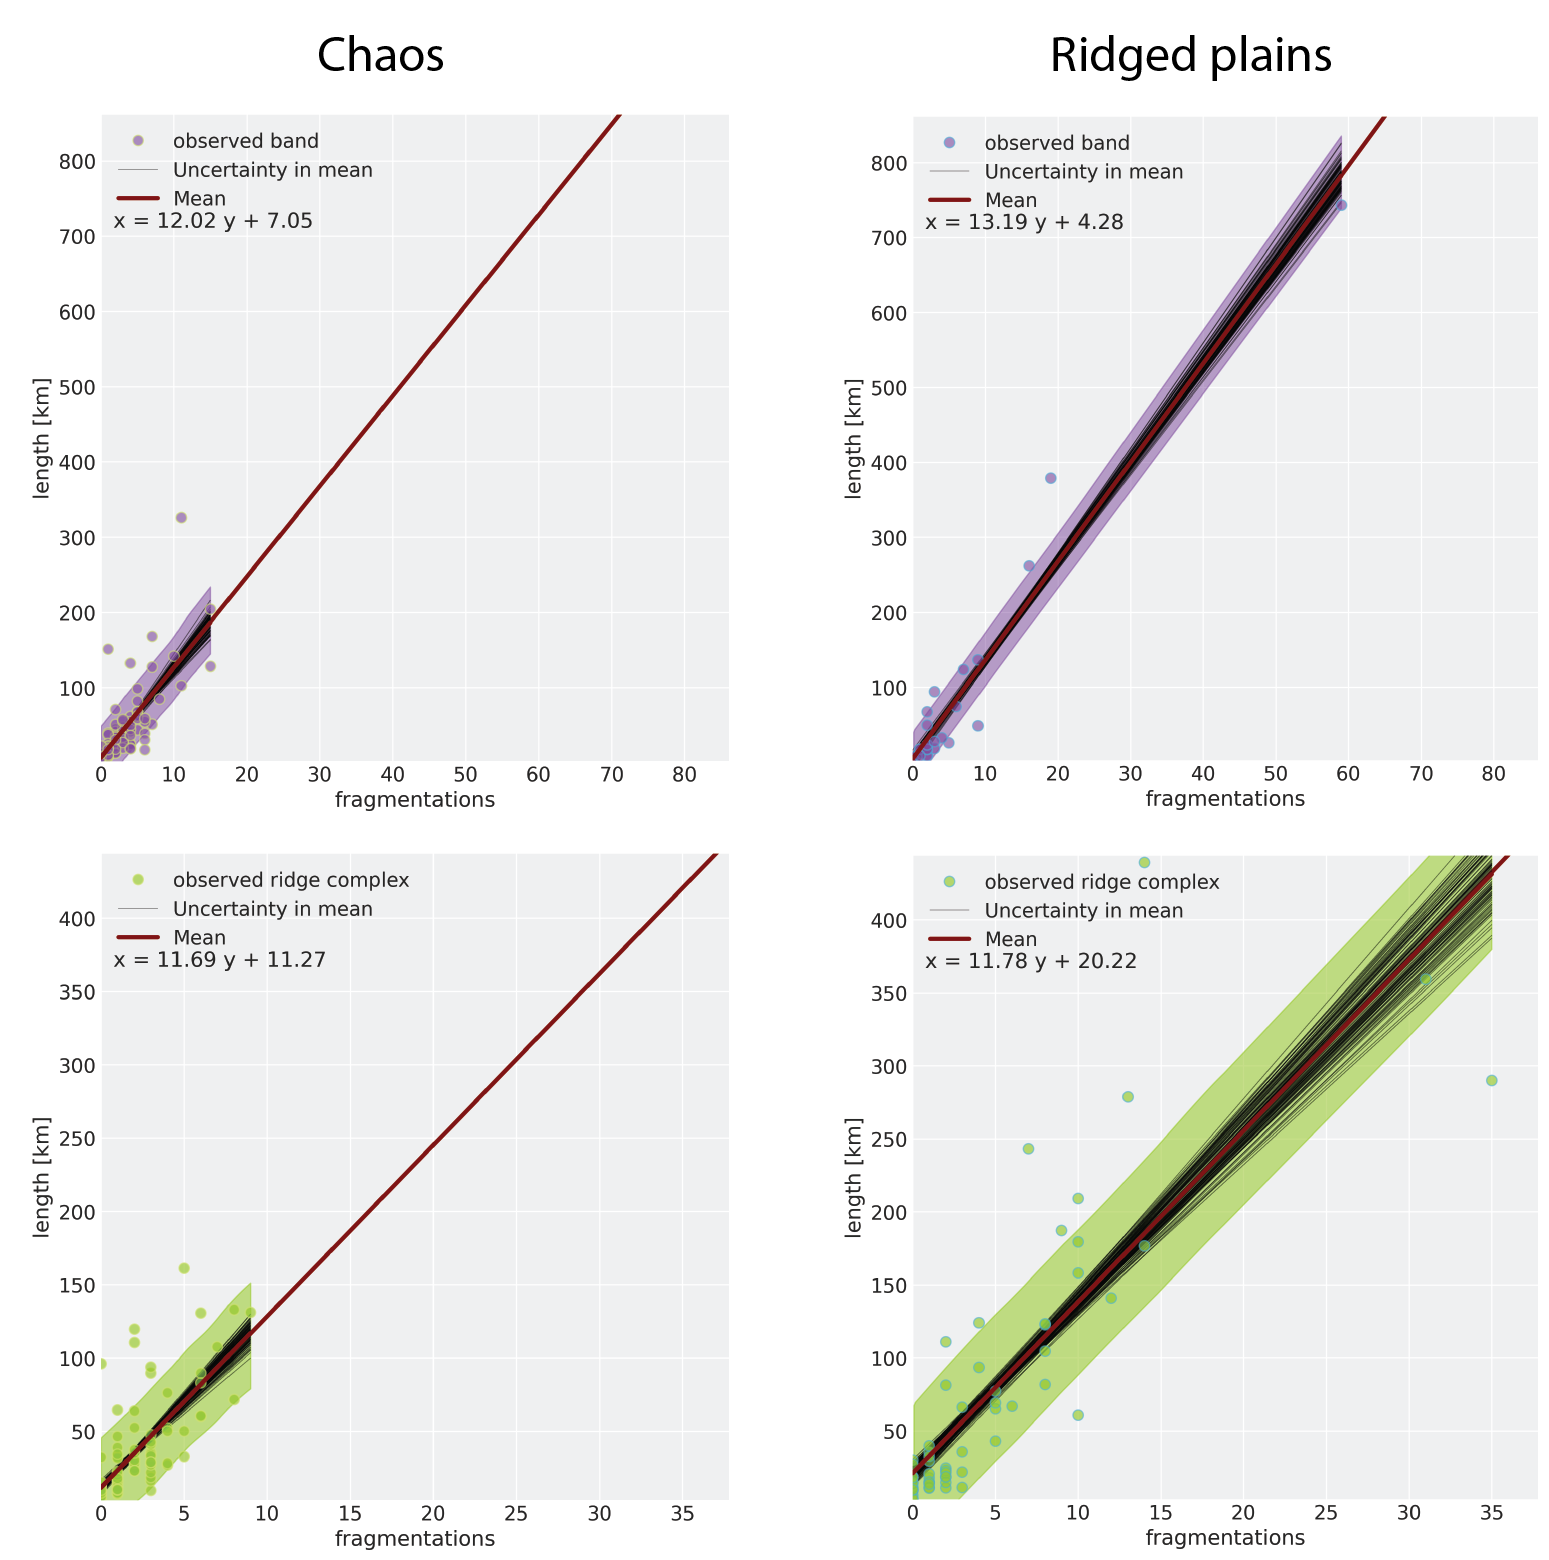
\includegraphics[width=\textwidth]{regional_mosaics/Figures/Bayes_analysis_regression_length_vs_fragm_band_rc.png}
%     \caption{Linear regression analysis for lineament length versus number of fragmentations, for \textbf{bands} and \textbf{ridge complexes}. The filled area shows the 97\% highest probability density interval of the posterior predictive samples (indicating where 97\% of the actual data are contained based on the posterior distribution).}
%     \label{fig_Bayes_length_frags_1}
% \end{figure*}
% \begin{figure*}
%     \centering
%     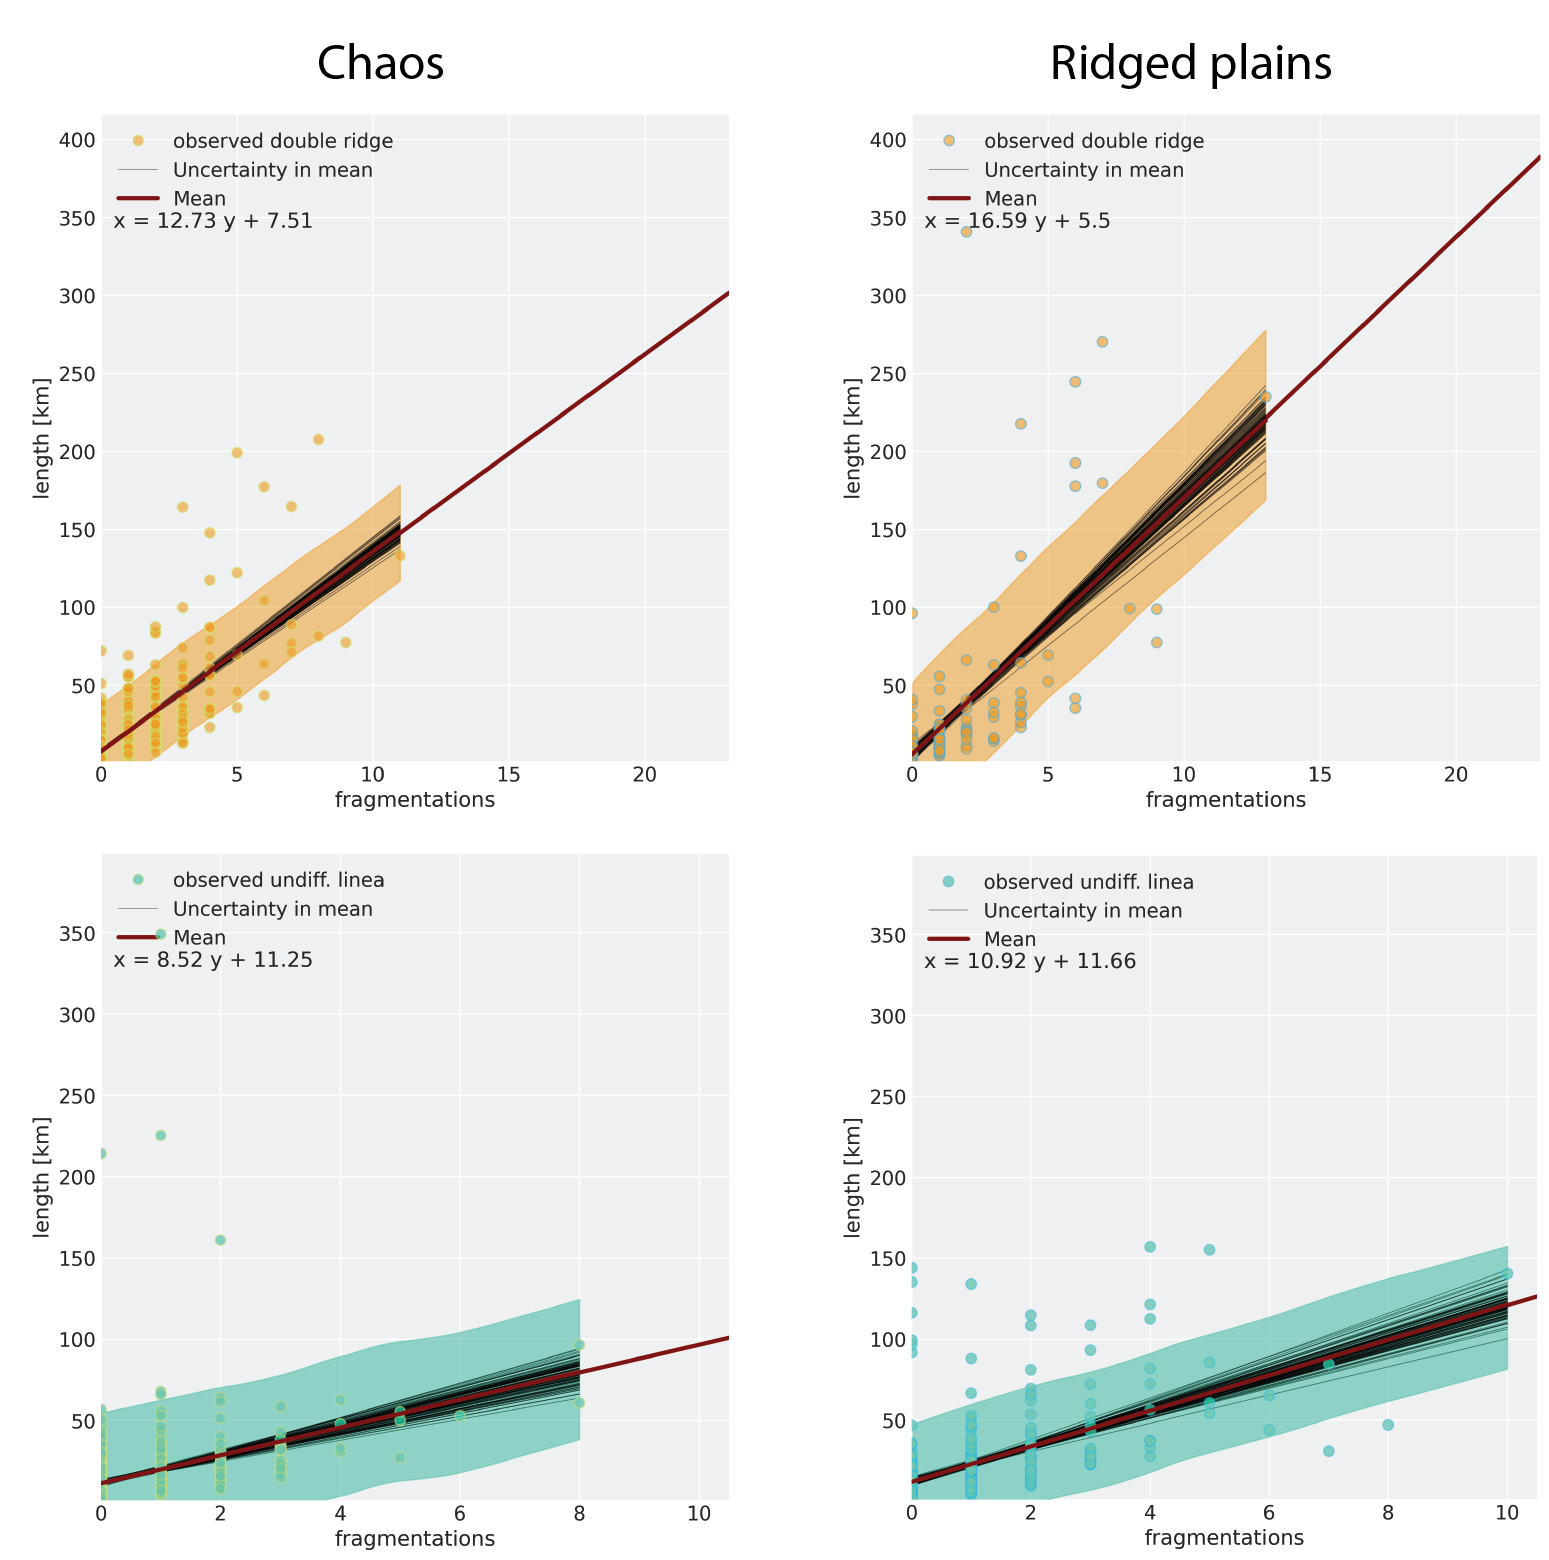
\includegraphics[width=\textwidth]{regional_mosaics/Figures/Bayes_analysis_regression_length_vs_fragm_db_ul.png}
%     \caption{Same as \Cref{fig_Bayes_length_frags_1} for \textbf{double ridges} and \textbf{undifferentiated lineae}.}
%     \label{fig_Bayes_length_frags_2}
% \end{figure*}
% 
% % legnth vs. FPK
% \begin{figure*}
%     \centering
%     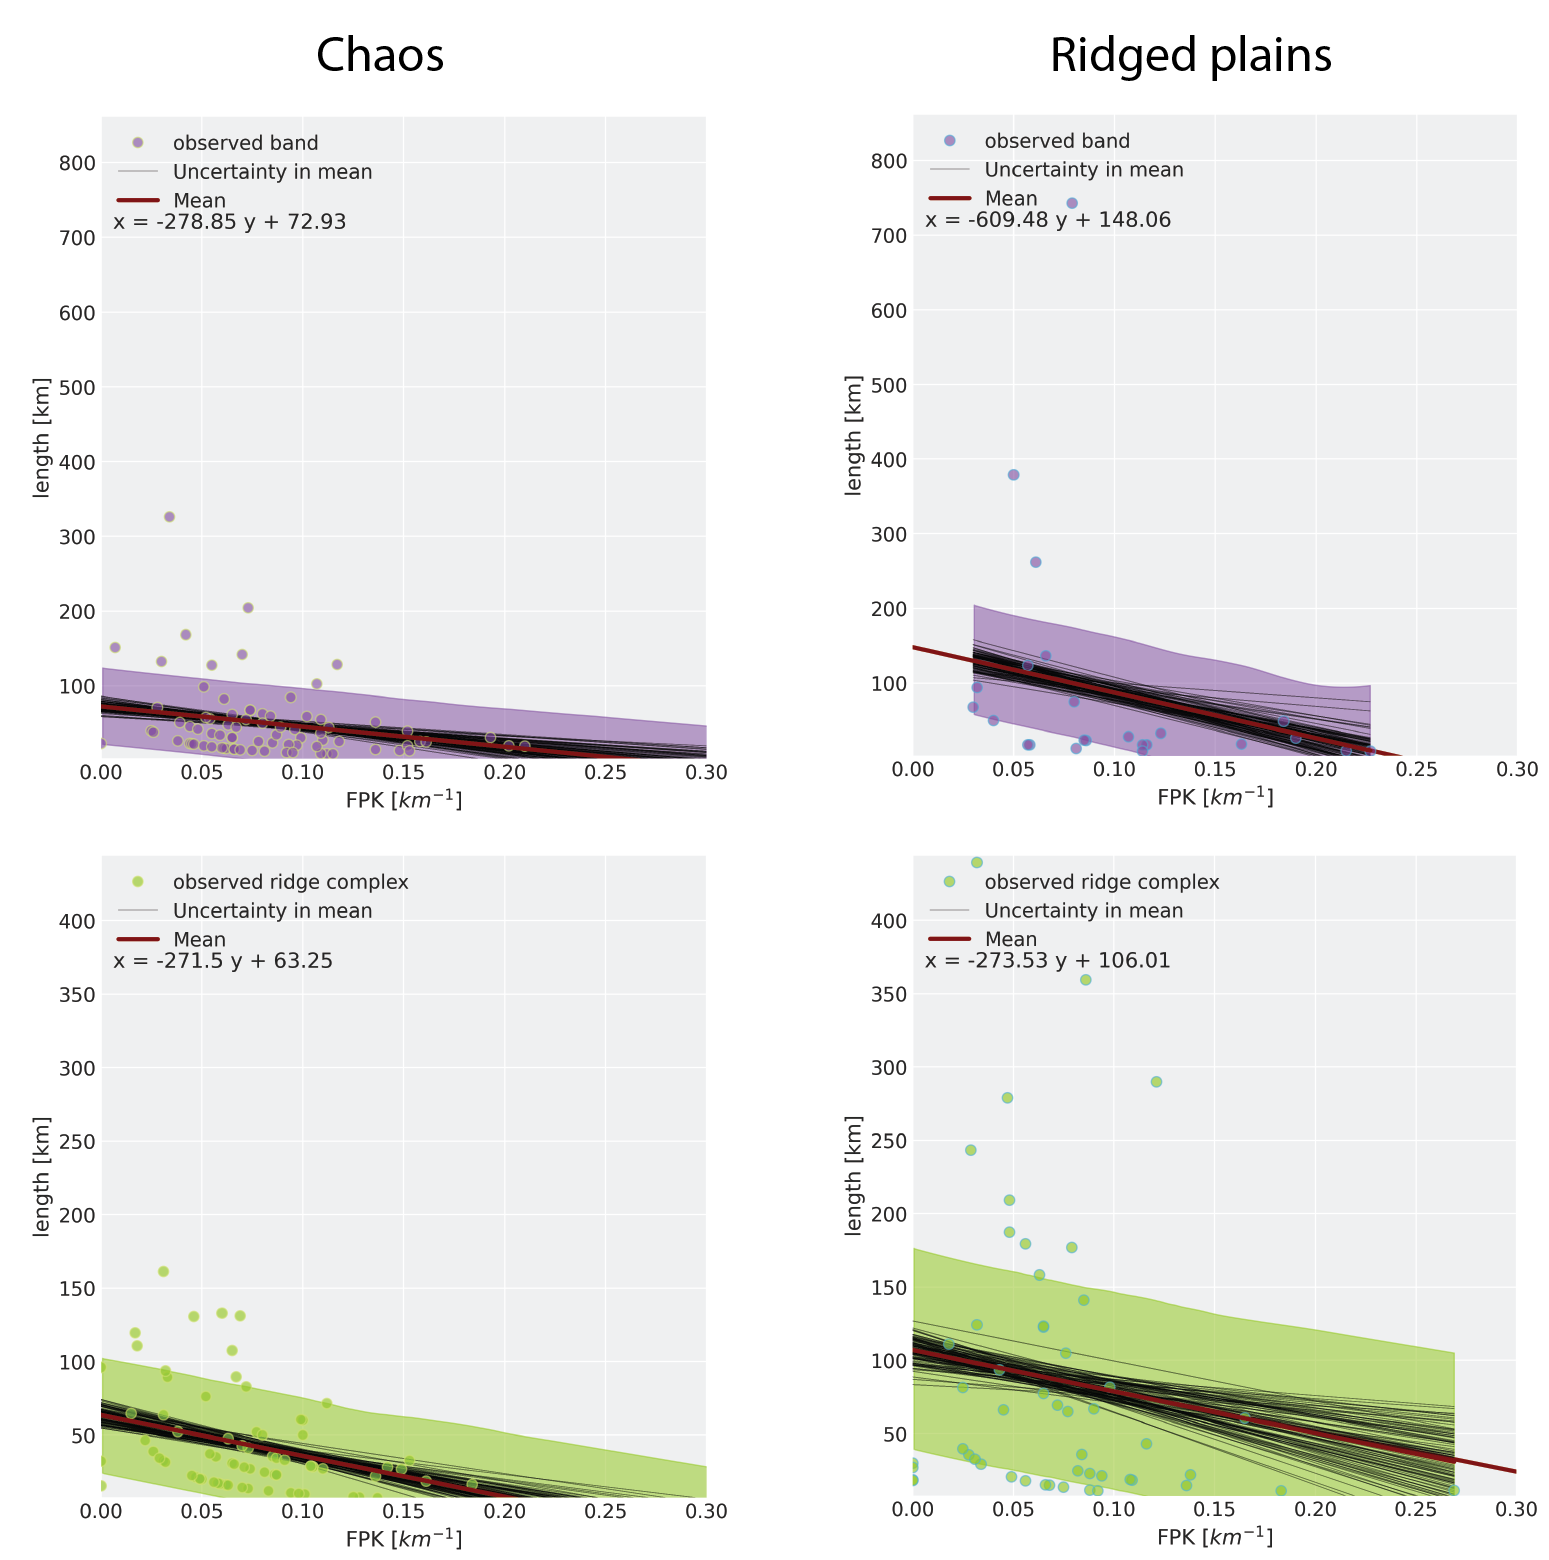
\includegraphics[width=\textwidth]{regional_mosaics/Figures/Bayes_analysis_regression_length_vs_FPK_b_rc.png}
%     \caption{Linear regression analysis for lineament length versus fragmentations per kilometre (FPK), for \textbf{bands} and \textbf{ridge complexes}. The filled area shows the 97\% highest probability density interval of the posterior predictive samples (indicating where 97\% of the actual data are contained based on the posterior distribution).}
%     \label{fig_Bayeslength_FPK_1}
% \end{figure*}
% \begin{figure*}
%     \centering
%     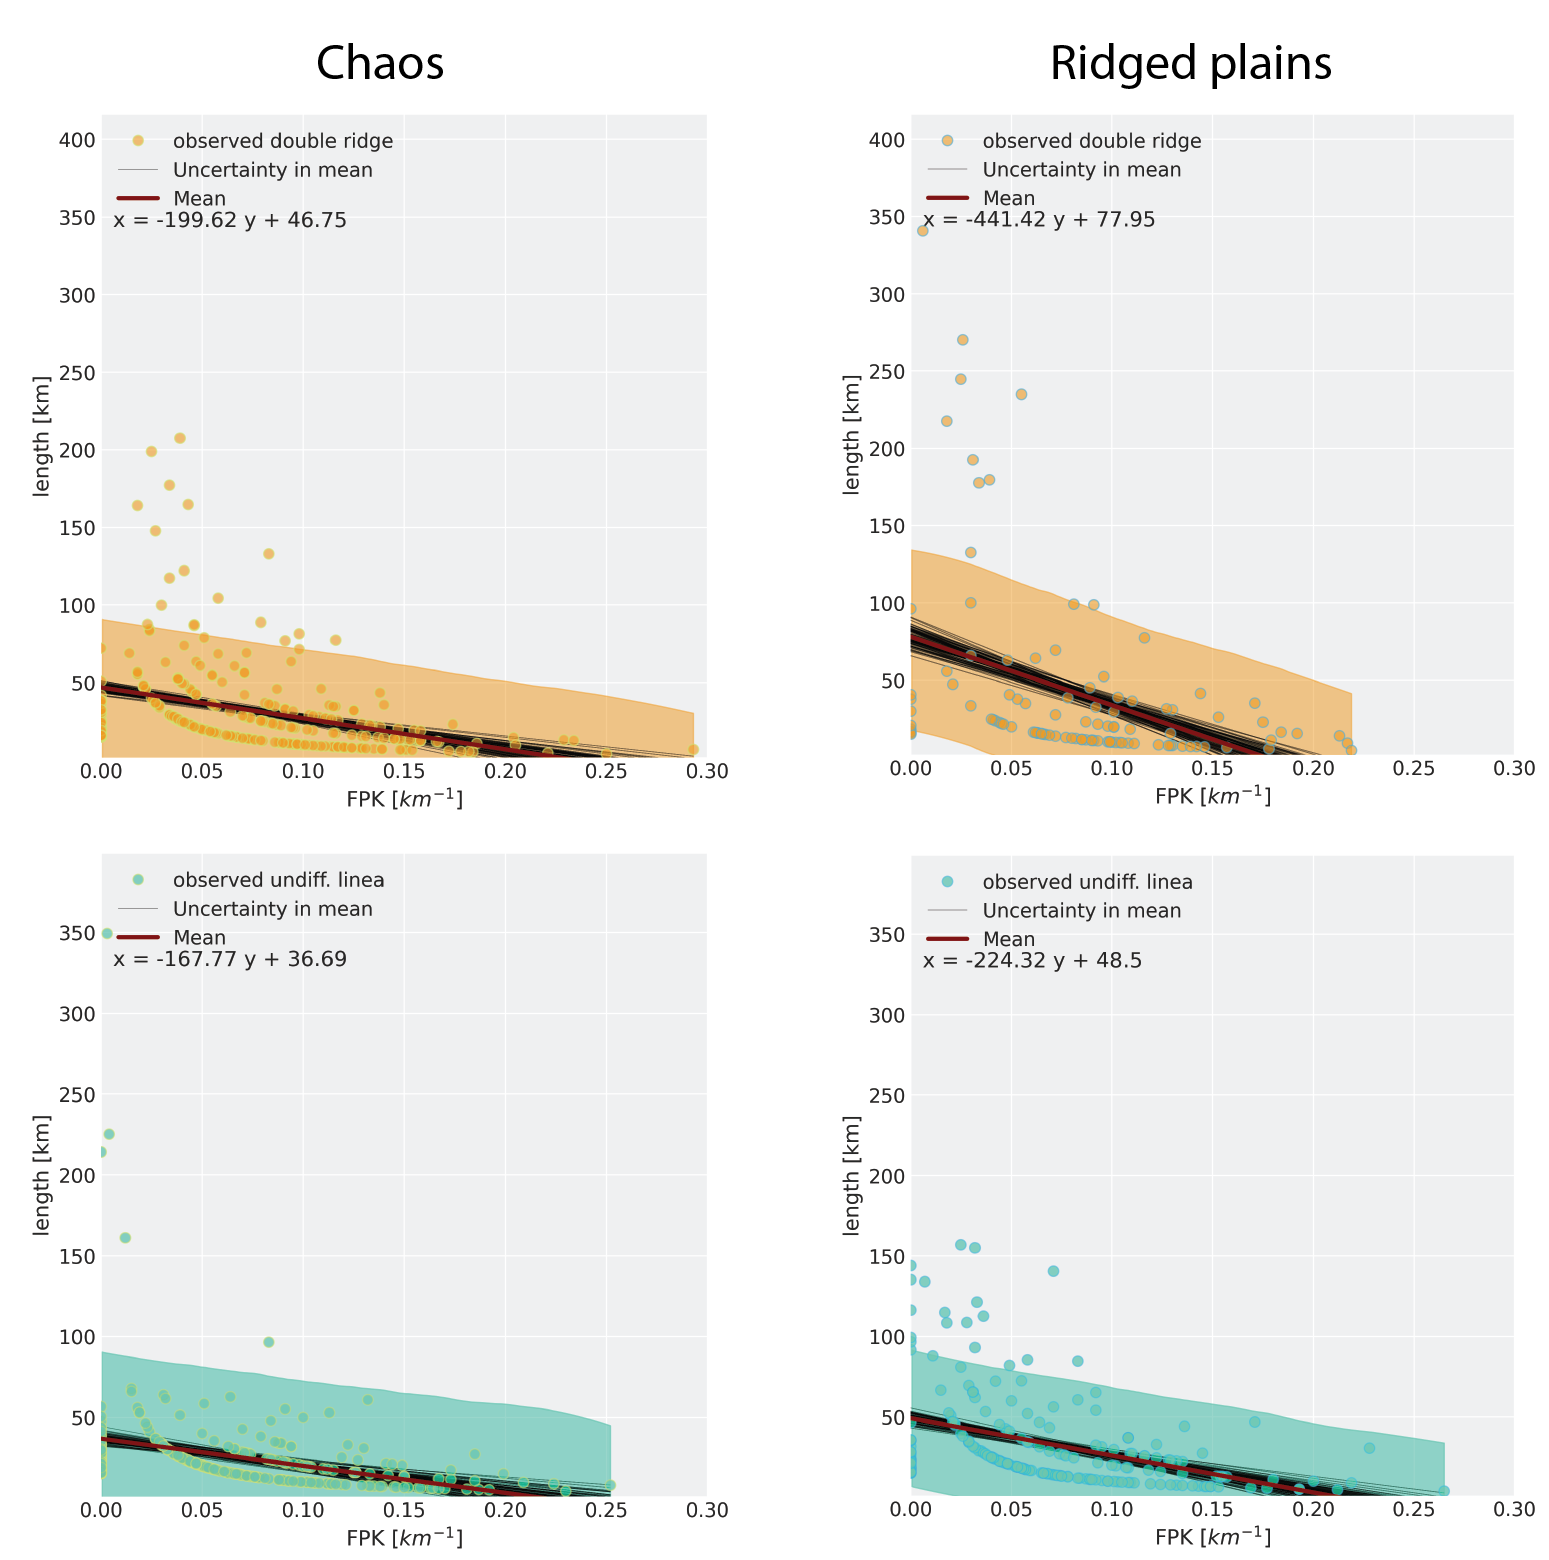
\includegraphics[width=\textwidth]{regional_mosaics/Figures/Bayes_analysis_regression_length_vs_FPK_db_ul.png}
%     \caption{Same as \Cref{fig_Bayeslength_FPK_1} for \textbf{double ridges} and \textbf{undifferentiated lineae}.}
%     \label{fig_Bayeslength_FPK_2}
% \end{figure*}
% 
% % width vs. FPK
% \begin{figure*}
%     \centering
%     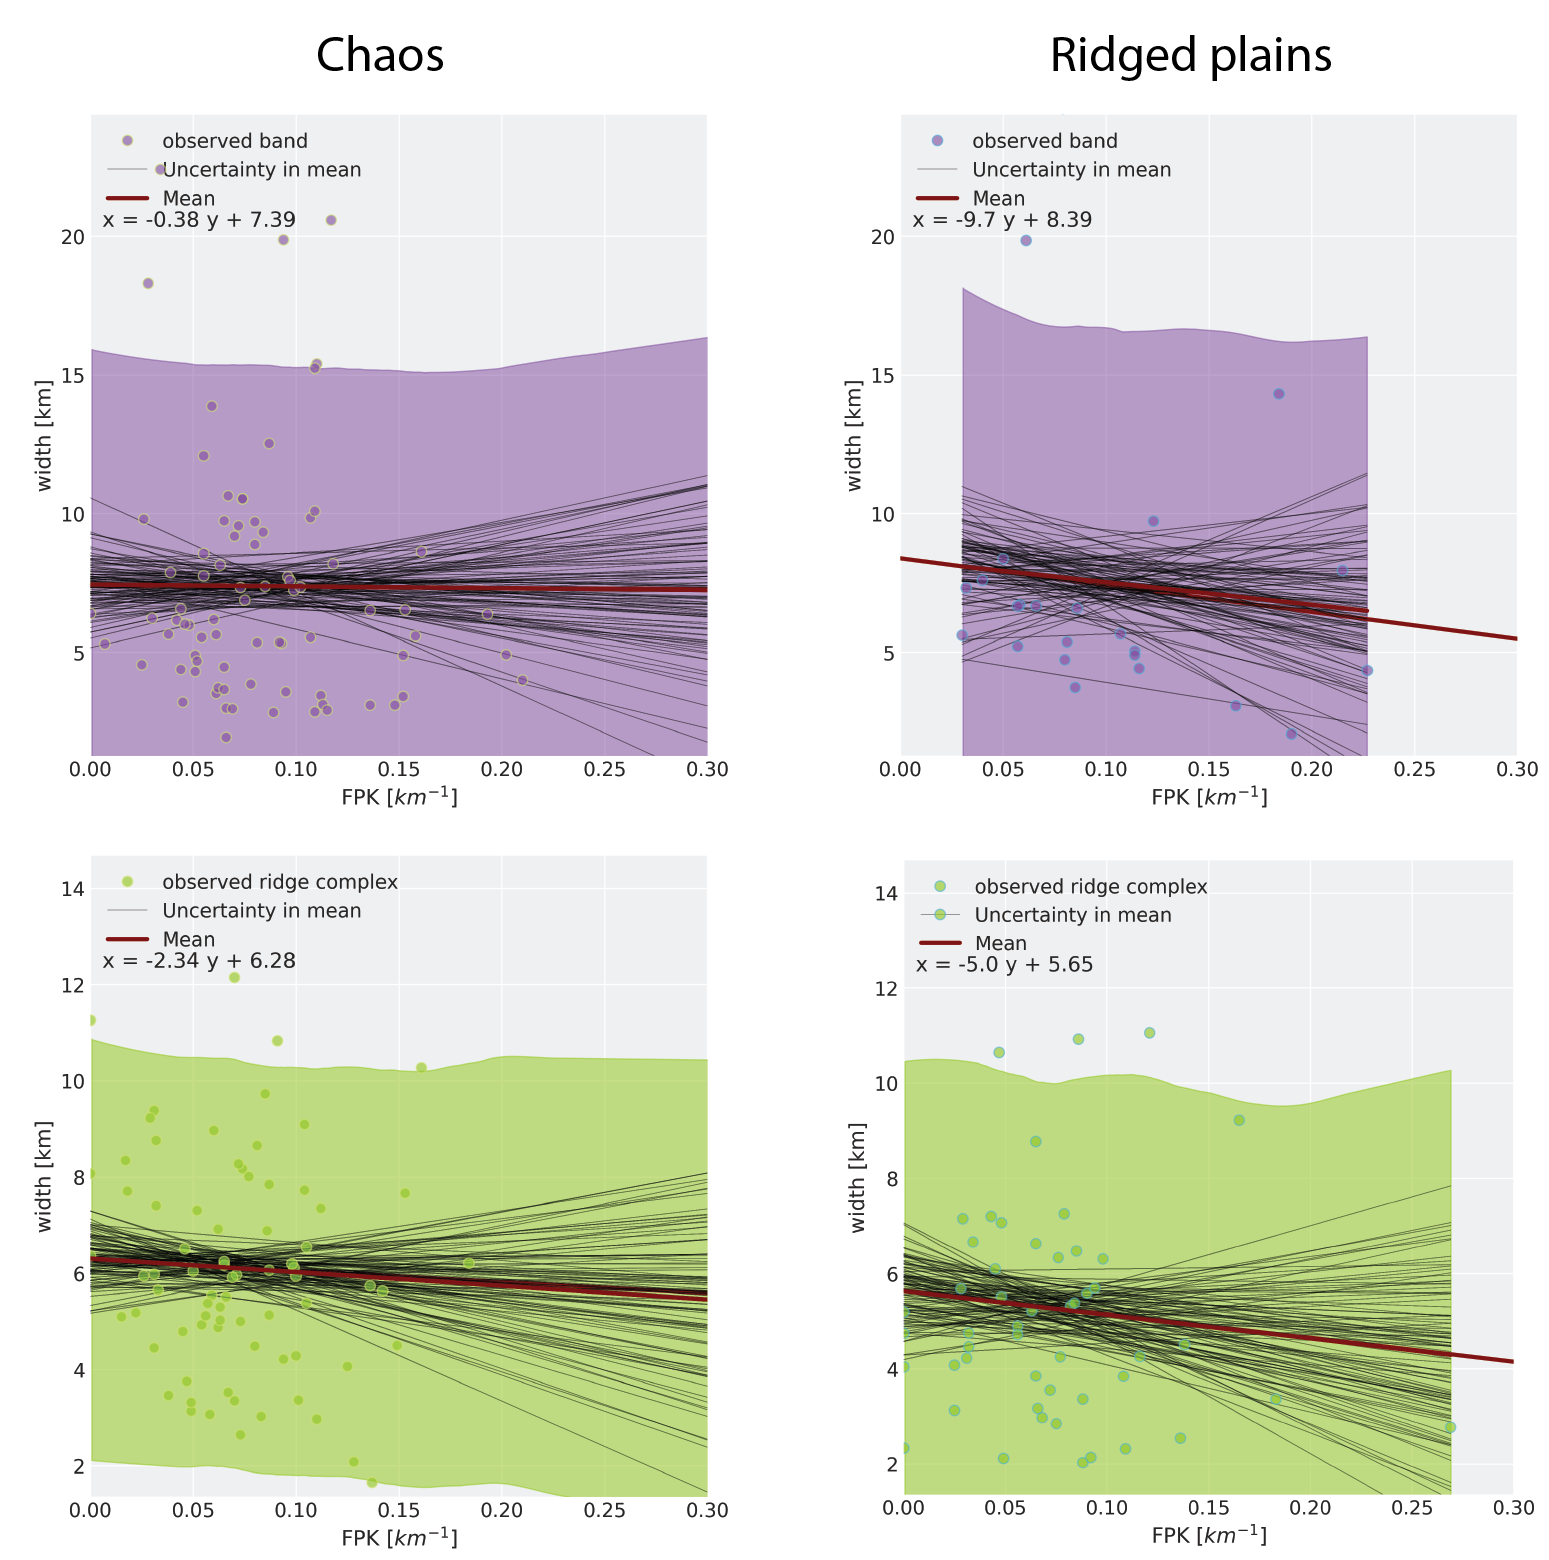
\includegraphics[width=\textwidth]{regional_mosaics/Figures/Bayes_analysis_regression_width_vs_FPK_b_rc.png}
%     \caption{Linear regression analysis for lineament width versus fragmentations per kilometre (FPK), for \textbf{bands} and \textbf{ridge complexes}. The filled area shows the 97\% highest probability density interval of the posterior predictive samples (indicating where 97\% of the actual data are contained based on the posterior distribution).}
%     \label{fig_Bayeswidth_FPK_1}
% \end{figure*}
% \begin{figure*}
%     \centering
%     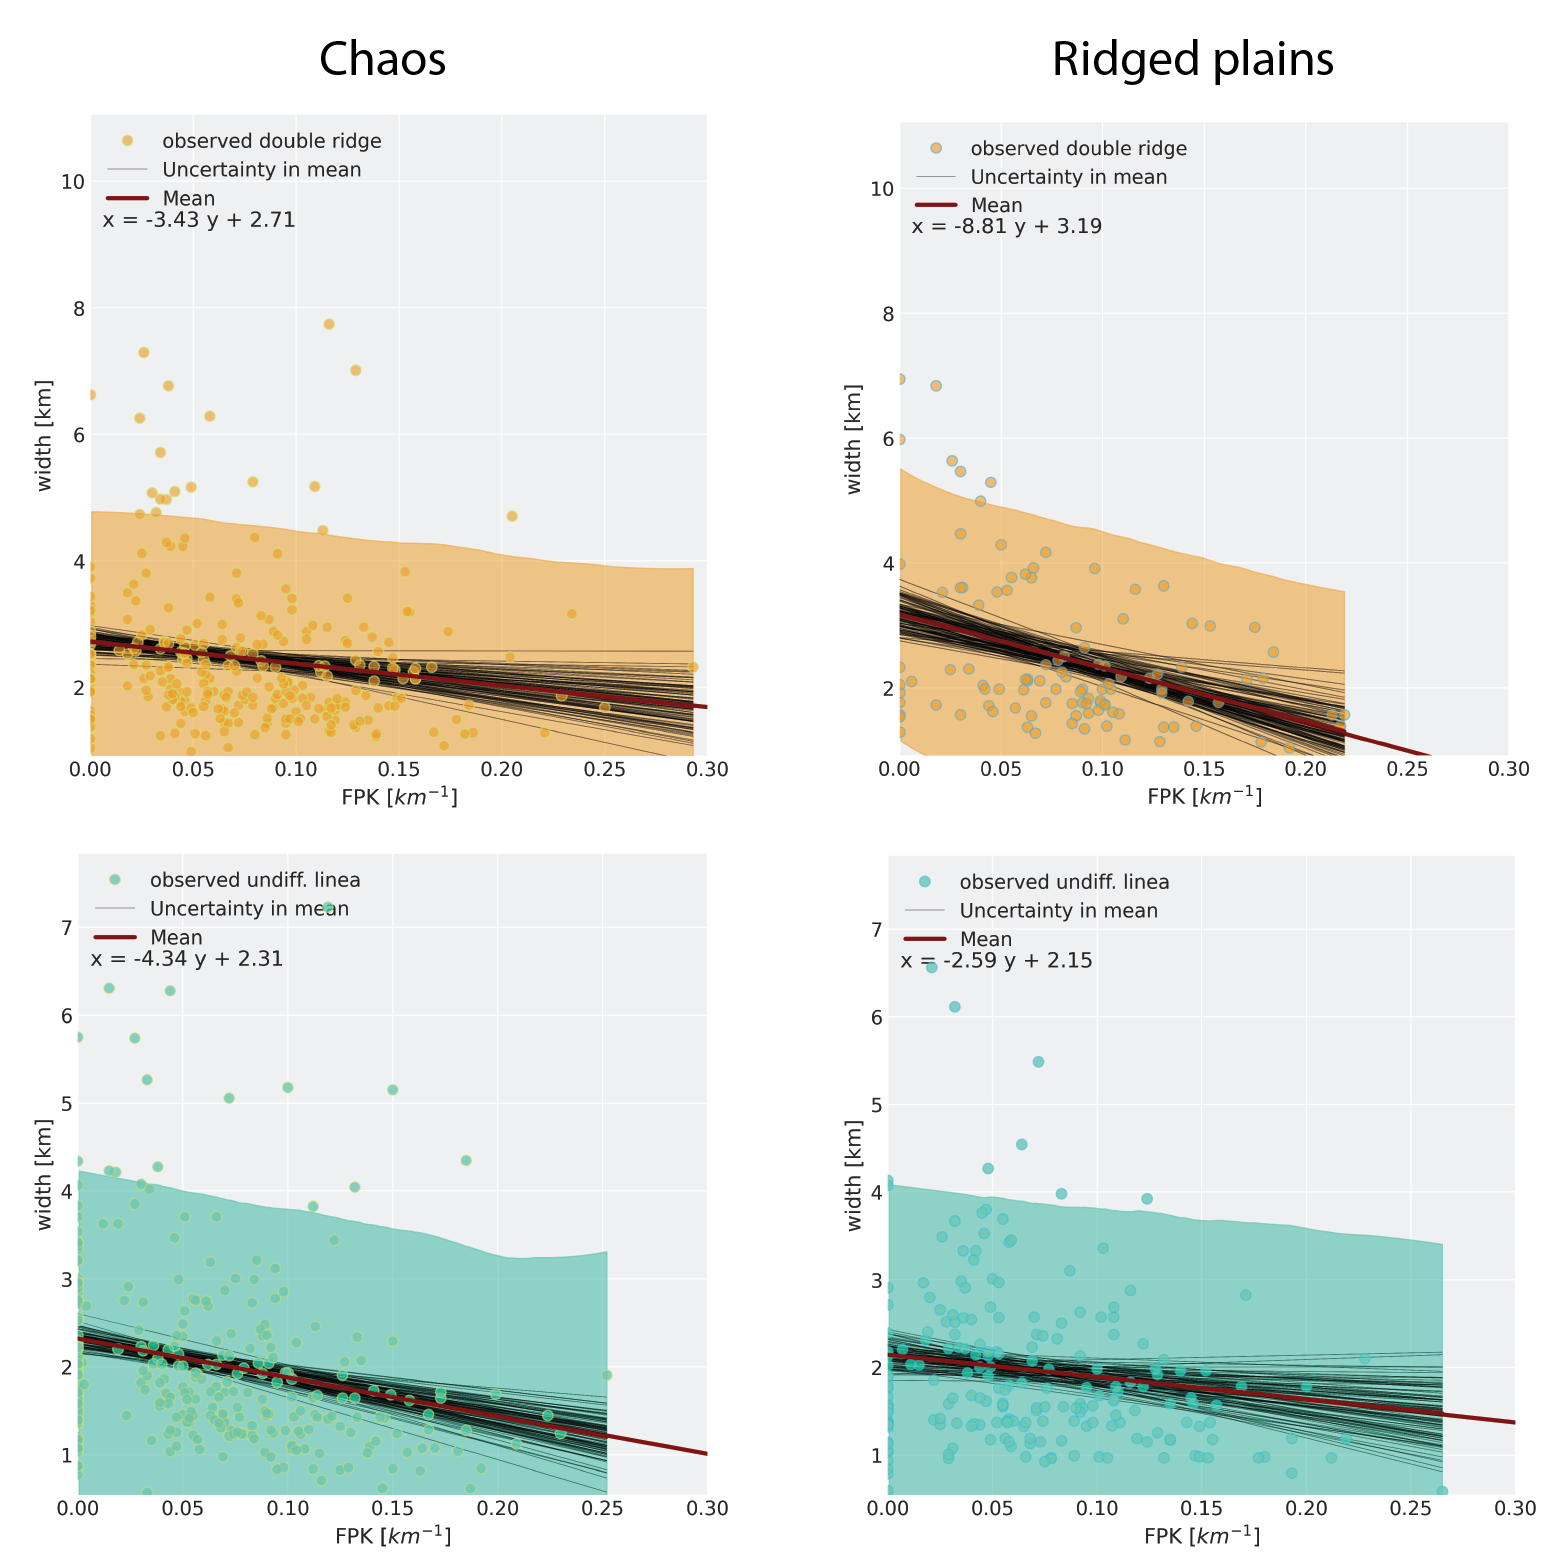
\includegraphics[width=\textwidth]{regional_mosaics/Figures/Bayes_analysis_regression_width_vs_FPK_db_ul.png}
%     \caption{Same as \Cref{fig_Bayeswidth_FPK_1} for \textbf{double ridges} and \textbf{undifferentiated lineae}.}
%     \label{fig_Bayeswidth_FPK_2}
% \end{figure*}
% 
% % width vs length
% \begin{figure*}
%     \centering
%     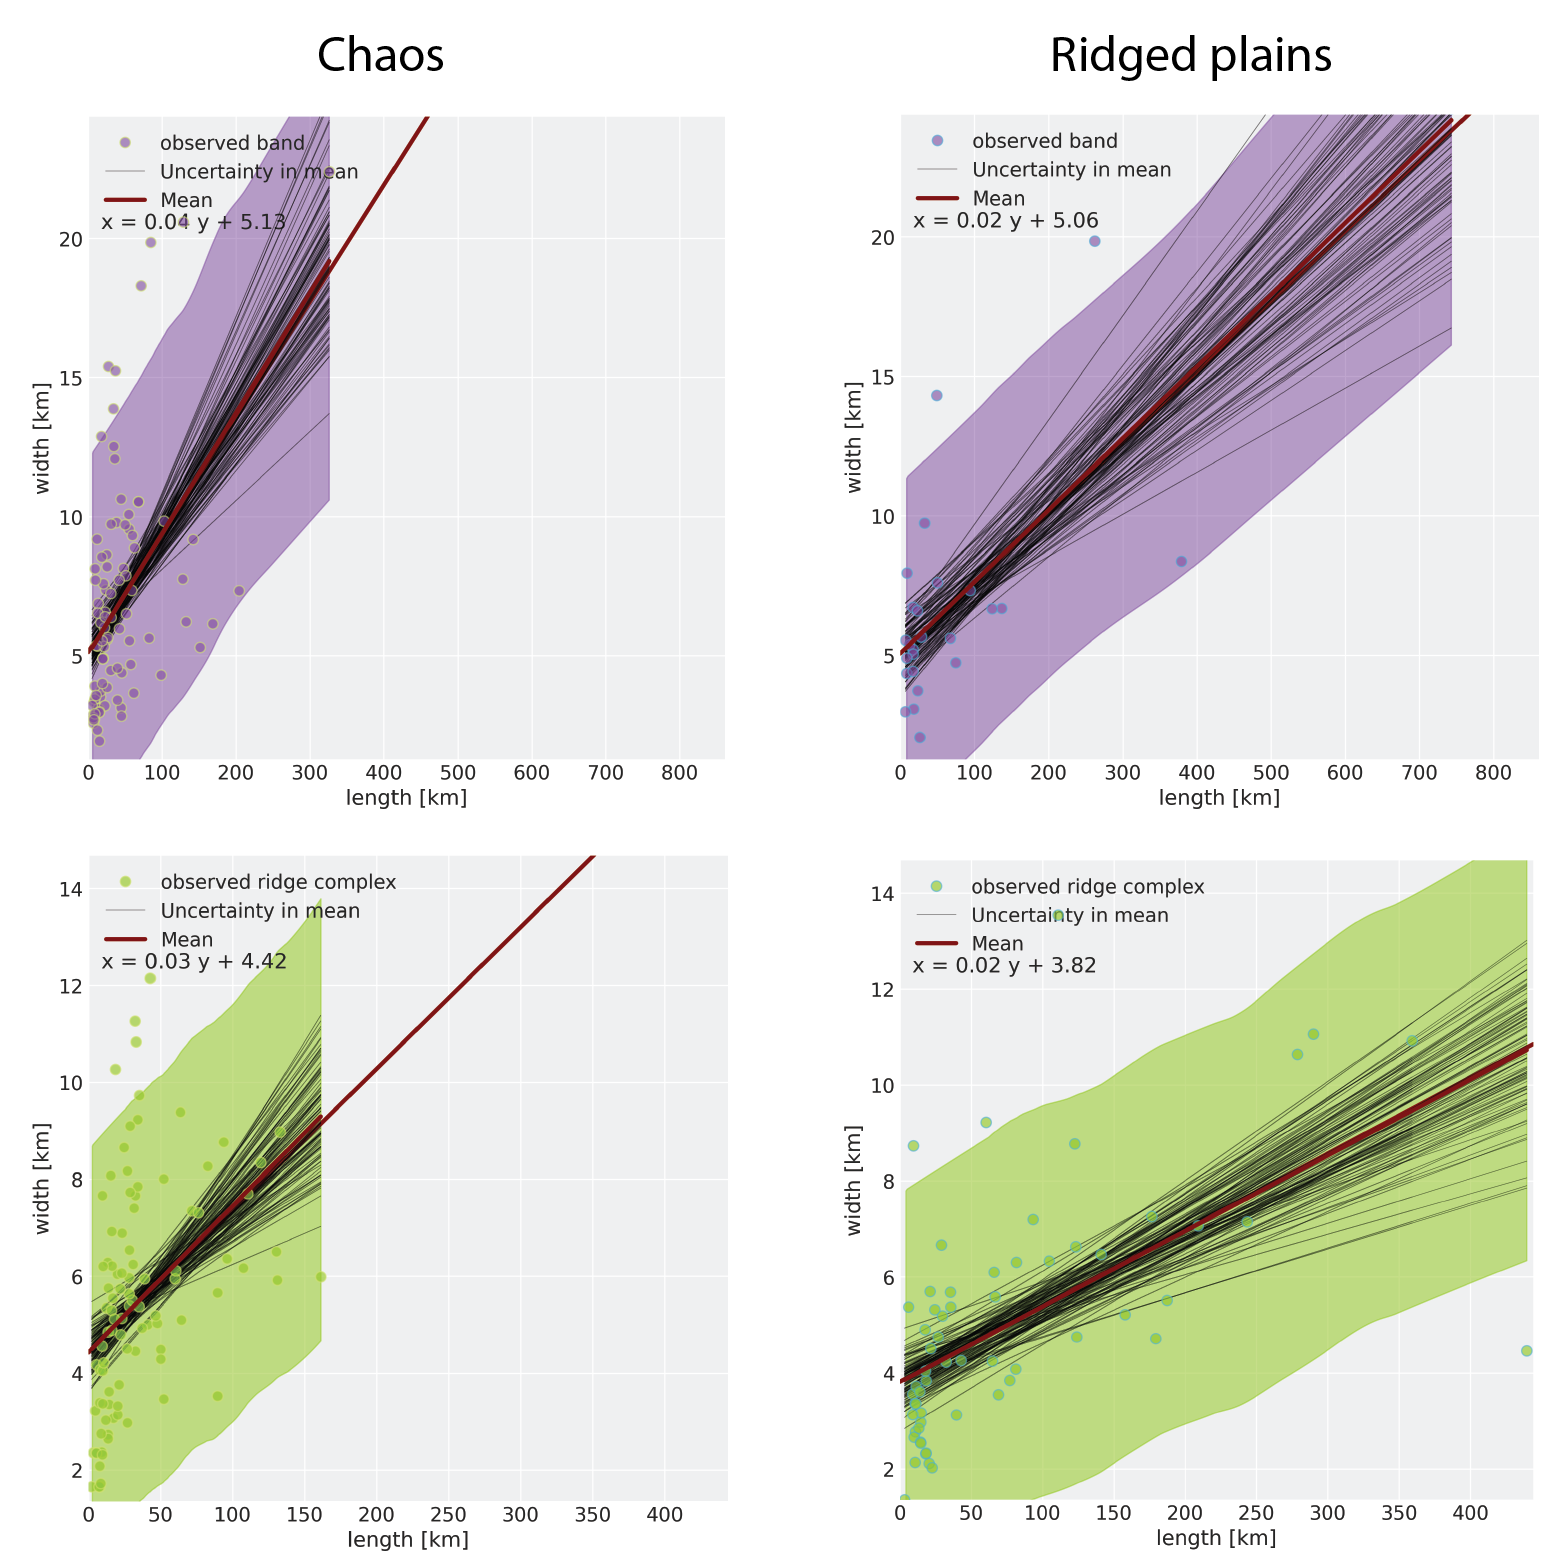
\includegraphics[width=\textwidth]{regional_mosaics/Figures/Bayes_analysis_regression_width_vs_length_b_rc.png}
%     \caption{Linear regression analysis for lineament width versus length, for \textbf{bands} and \textbf{ridge complexes}. The filled area shows the 97\% highest probability density interval of the posterior predictive samples (indicating where 97\% of the actual data are contained based on the posterior distribution).}
%     \label{fig_Bayeswidth_length_1}
% \end{figure*}
% \begin{figure*}
%     \centering
%     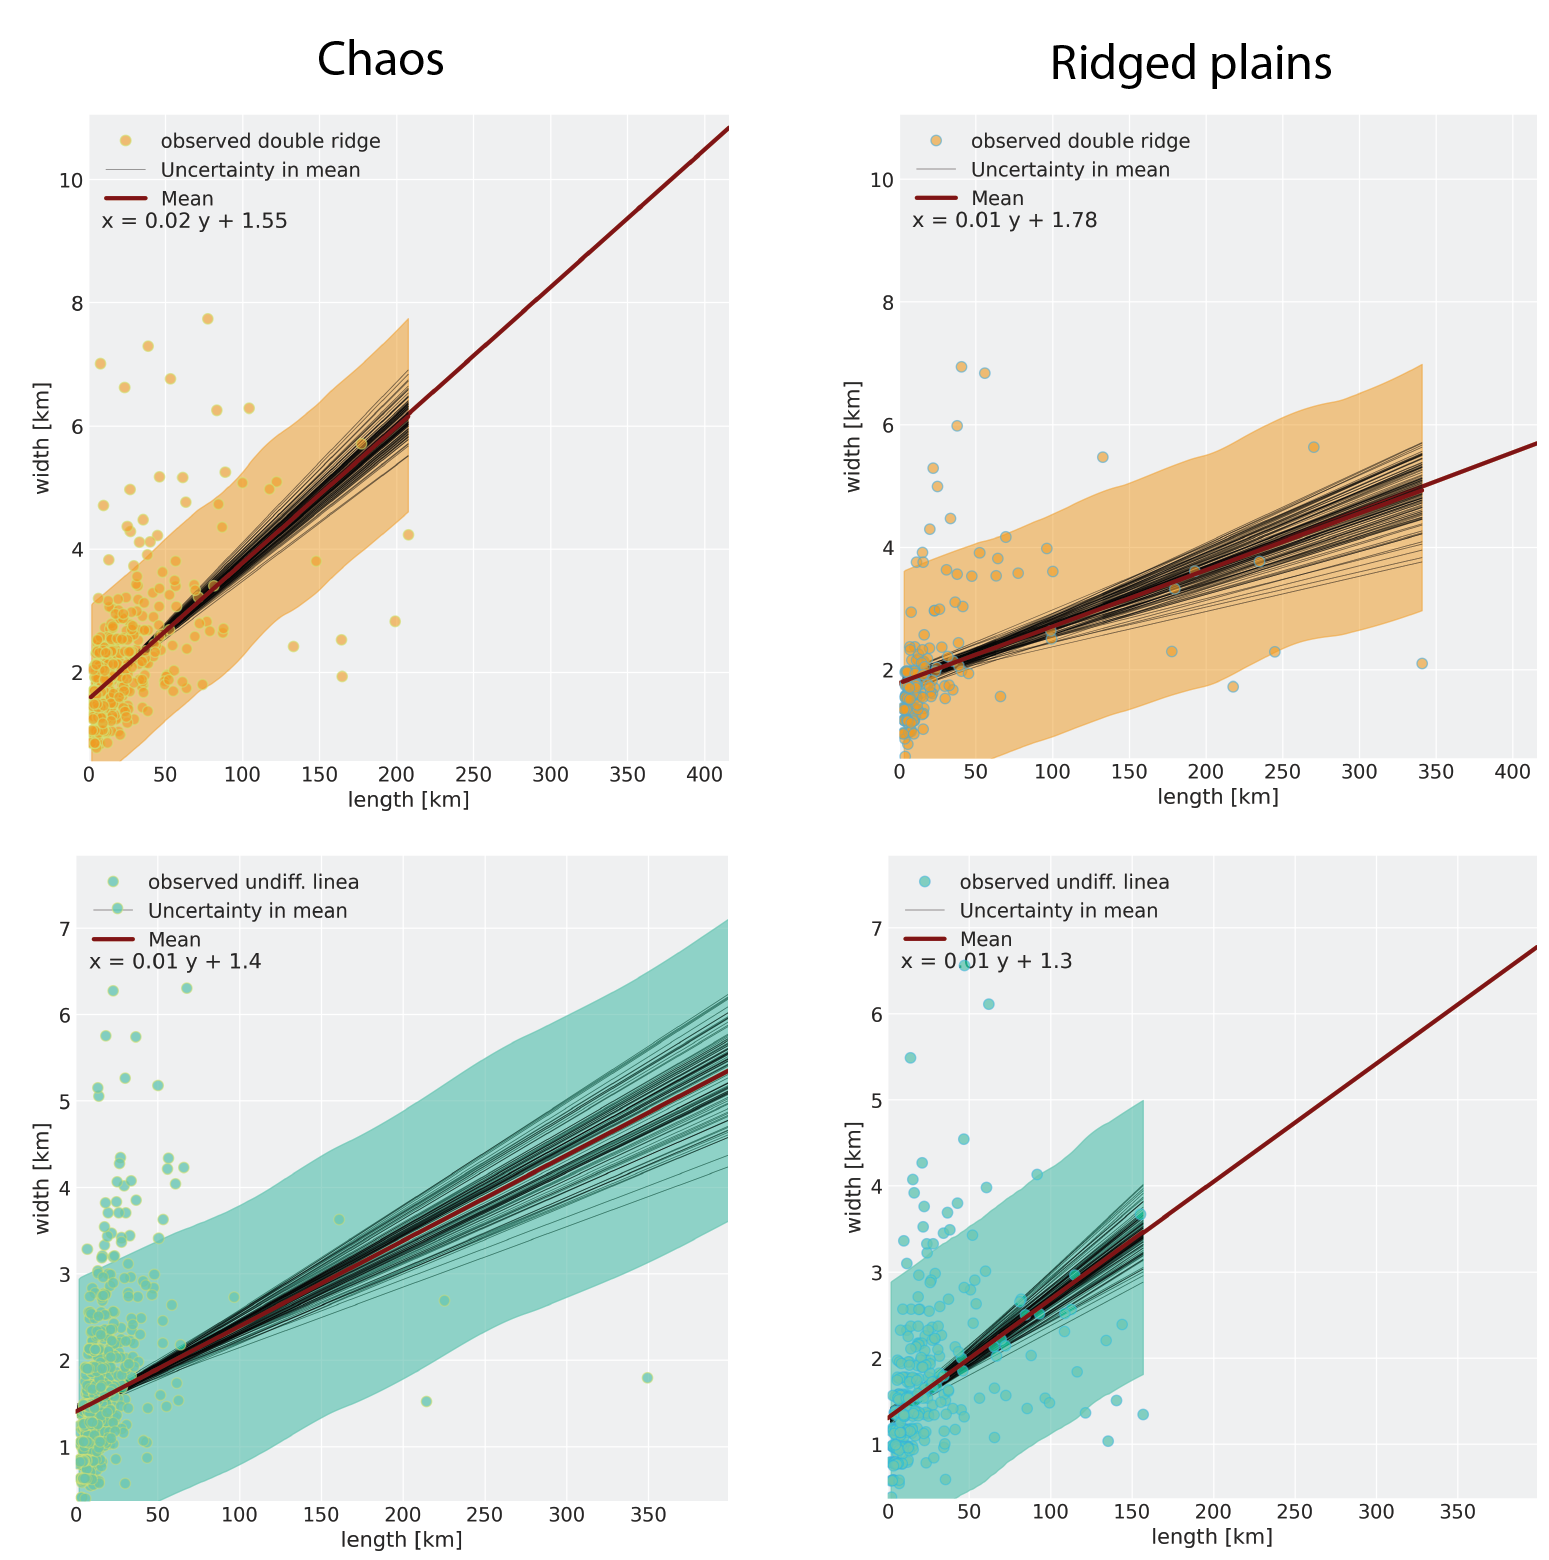
\includegraphics[width=\textwidth]{regional_mosaics/Figures/Bayes_analysis_regression_width_vs_length_db_ul.png}
%     \caption{Same as \Cref{fig_Bayeswidth_length_1} for \textbf{double ridges} and \textbf{undifferentiated lineae}.}
%     \label{fig_Bayeswidth_length_2}
% \end{figure*}


\paragraph{\textbf{Do we find correlations between lineament characteristics, and do the fits vary for the chaos and ridged plains unit?}} Short answer: We find a weak correlation between relative age and width (younger lineaments seem to be wider). Separated into categories, we find that wider linea are longer. Together, this shows that young lineaments are more likely to be long and wide, which could be an observation bias due to fading and fragmentation. The fits only slightly vary for chaos vs ridged plains.

In the following, we analyse how the extracted characteristics correlate with each other. We note that for correlations with FPK, we filtered out values with FPK$=$0 \textbf{and} length $<$30~km, because these lineaments might either be old and fragmented or young.

\paragraph{Length vs number of fragmentations:} 
The Bayesian linear regression fit of length versus number of fragmentations (Figs.~12 and~13 in the original publication) shows that for most lineaments, a linear correlation of length and number of fragmentations provides a good fit. The slopes are flattest for undifferentiated lineae. Chaos and ridged plains show significant differences in slopes for double ridges and undifferentiated lineae when compared category-wise\sidenote{As shown in Table~17 in the supplementary material of the original publication.}. The ranges of slopes for different categories (9.6 to \qty{14.7}{\km}) are higher than between chaos and ridged plains (max. \qty{4}{\km} difference in slope, for double ridges).

\paragraph{Length vs FPK:} 
We would expect to see no correlation for length vs. FPK (Figs.~14 and~15 in the original publication), if the number of fragmentations is positively correlated to the number of fragmentations. However, we observe a residual, negative correlation of length with FPK, simply because not all lineaments lie on one line. More values with a low FPK lie outside the 97\% highest probability density interval (HDPI), which should capture 97\% of the distributed data. Since the number of fragmentations is discrete, we see constant, exponentially decreasing lines. The negative correlation means that longer linea are disproportionally young, which is either an observation bias, potentially due to fading\sidecite{Bierhaus2009}, or a bias from connecting lineaments, if heavily fragmented lineae are too fragmented to show their continuation. Overall, chaos shows slopes closer to zero than ridged plains. The closest to a slope of zero get undifferentiated lineae in chaos terrain. The maximal negative slope is exhibited by bands in ridged plains.

\paragraph{Width vs FPK:} 
Correlating width with FPK (Figs.~16 and~17 in the original publication) tries to answer the question: Are older lineaments wider or narrower? In general, older lineaments seem to be narrower, but the uncertainty is large and there might be no underlying real-world correlation. The most constrained negative correlation is exhibited by double ridges in ridged plains. Slopes for bands and ridge complexes range from negative to positive within their 97\% HDPI, for both chaos and ridged plains. The slopes of double ridges and undifferentiated are negative within their 97\% HDPI. The negative correlation, after an observational bias indicated by length vs FPK is excluded, could either indicate that more recently formed double ridges and undifferentiated lineae develop into wider lineaments, or that throughout the evolution of double ridges and undifferentiated lineae, the width decreases, hinting at the possibility of subduction or shrinking (also in the vertical) due to a weakening of driving forces, such as changing shear forces\sidecite{Gaidos2000, Nimmo2002, Han2008}.

\paragraph{Width vs length:} A possible correlation of width with length can answer the question: Are longer lineaments also wider? Or are longer lineaments narrower?  We find that, separated into categories, longer linea are wider (Figs.~18 and~19 in the original publication). However, the scatter plots show a wide range of widths for short lineaments, which is not fully captured by the linear regression line, but only in the HDPI. If longer lineaments ($>$\qty{50}{\km}) would be excluded, correlations would be weaker. This means that short lineaments can have any width, while long lineaments are not especially narrow. Nevertheless, slopes are higher (longer lineaments are even wider) in chaos terrain, although the comparison is flawed by the fact that lineaments in chaos terrain are generally shorter. The effect of longer and wider lineaments is most pronounced for bands in chaos terrain. We speculate that if the ice fails in a way that allows a long crack to result (e.g. if a higher pressure builds up for a long crack to form), the crack might also penetrate deeper than shorter cracks, which could result in wider lineaments, because the crack stays active for longer. However, this preliminary result needs to be validated, for example with lineament age sequences to better quantify the relation of age and length.\\

The scatter plots in Figs.~16 and~17 in the original publication show in more detail than \Cref{fig:grid_chaosvspr}.c that the FPK reaches higher values in chaos terrain.

\subsubsection{Discussion of the revised lineament map}\label{sec:discussing_revisedMap}
The question that arose most often during revision of the southern leading hemisphere RegMap 17ESREGMAP02 was about the differentiation of bands and ridge complexes. For one, morphologies of ridged bands and ridge complexes are similar, while other types of bands, e.g. smooth bands\sidecite{ProckterPatterson2009}, are distinct. Adding band sub-categories to LineaMapper might help to increase performance, although increasing number of categories does not always lead to better classification. Since some bands appear bright in infrared wavelengths\sidecite{DoggettEuropaBook2009}, LineaMapper could be trained to take in spectral information, for example from Galileo Near Infrared Mapping Spectrometer (NIMS) observations. During the Europa Clipper mission, EIS can be combined with spectral data from the Mapping Imaging Spectrometer for Europa\sidecite{Blaney2022} datasets could be combined and input together into LineaMapper.

Furthermore, a finer distinction of band types would lead to further statistical insights. With the current categorisation, we observe similar distributions for bands-ridge complexes and double ridges-undifferentiated lineae. This could imply that most undifferentiated lineae would resolve as double ridges or share the same formation mechanism, while for bands and ridge complexes, they are either hard to distinguish by their morphologies or form similarly\sidecite{Patterson2010}. 

However, there is one interesting difference to ridge complexes. The fact that bands are widest and have the highest FPK values, which means they are on average oldest, might indicate that bands formed earlier and became wider than any other category. % This result is in line with .

We characterize the nature of fragmentation processes in ridged plains and chaos terrain.
We find higher chaos vs. ridged plains differences for bands and ridge complexes than for undifferentiated lineae and double ridges. Most striking is the almost identical width distribution of undifferentiated lineae and double ridges.
Together with the observation of an absence of young bands in ridged plains, we hypothesise that more recently formed features survive disruption during chaos formation better, maybe simply because they have locally the highest elevation, or the composition and porosity withstands chaos disruption more likely. However, it could also be that older lineaments blend in easier with the chaos matrix, which leads to an observational bias.  

The slopes of length fit by number of fragmentations could be taken to work out a refined, category-wise FPK, which could capture the differences in how lineaments are fragmented. The exponentially decreasing slopes of length vs FPK could tell us that the FPK should rather be calculated by the length divided by the logarithm of the number of fragmentations. On the other hand, this might be an observational bias, likely due to resolution, which prevents a full record of fragmentations. A higher resolution dataset will shed light on this matter. The possible negative correlation of width vs FPK (younger lineaments are wider) needs verification with an established age sequence. The positive correlation of width with length (longer linea are wider) could be confirmed on other parts of the RegMaps, and possible explanations should be investigated.
We note that, as a preliminary result, we do not find any significant correlation of radiance with FPK for any category when we evaluate the photometrically corrected images (not shown).

We empirically find that fine cracks (troughs) can be identified by filtering for undifferentiated lineae with a length greater than 150~km. Out of these long cracks, the youngest ones can be identified by width $\leq$ 3~km and FPK $<$ 0.03 fragmentations per kilometer. With this, LineaMapper will be useful for recent trough identification in EIS images.

\plainwidefig{1}{regional_mosaics/Figures/LM1_1_polygon_foroverleaf.png}{Fully-automatically produced lineament map of the Galileo RegMaps with \textbf{LineaMapper v1.1}. A) RegMap of the anti-jovian, trailing hemisphere. B) RegMap of the leading hemisphere. The absence or reduced density of lineaments concurs with the presence of chaos terrain. C) Excerpt of the leading hemisphere. A unit of chaos terrain is left blank, i.e. LineaMapper does not confuse chaos terrain with lineaments here. D) Excerpt of the trailing hemisphere with all four categories predicted by LineaMapper.}{fig:raw_regmaps_LM1.1}


\plainwidefig{1}{regional_mosaics/Figures/LM2_0_polygon_foroverleaf.png}{Fully-automatically produced lineament map of the Galileo RegMaps with \textbf{LineaMapper v2.0}. A) RegMap of the anti-jovian, trailing hemisphere. B) RegMap of the leading hemisphere. The absence or reduced density of lineaments concurs with the presence of chaos terrain. C) Excerpt of the leading hemisphere. A unit of chaos terrain is left blank, i.e. LineaMapper does not confuse chaos terrain with lineaments. D) Excerpt of the trailing hemisphere with all four categories predicted by LineaMapper.}{fig:raw_regmaps_LM2.0}

\subsubsection{Fully automatic RegMaps lineament map}\label{sec:fullRegMaps}

Based on tests with photometrically corrected input data, we decide to use the 149 non-corrected 'native' Galileo SSI images that constitute the RegMaps for inference with LineaMapper v1.1 and v2.0. The stitched LineaMapper output on the RegMaps is shown in \Cref{fig:raw_regmaps_LM1.1} for v1.1 and in \Cref{fig:raw_regmaps_LM2.0} for v2.0. The two predictions are qualitatively similar. This also manifests in the resulting number of predictions: we retrieve 133,801 stitched predictions with LineaMapper v1.1 and 134,101 predictions with LineaMapper v2.0. As an example, LineaMapper v1.1 needed 6 minutes for prediction and stitching of Galileo image with SSI ID \textit{C0449961814R} on one CPU. 

\plainwidefig[t]{1}{regional_mosaics/Figures/trailing_geounits.png}{Predicted geological units (chaos, transition unit, ridged plains) on the trailing RegMap by the lineament density extracted from LineaMapper v1.1 and v2.0 predictions. For comparison, the global geologic map~\cite{Leonard2024} is shown on the right with the outline of the analyzed SSI images.}{fig_trailing_chaos_pr_predicted}

\plainwidefig[t]{1}{regional_mosaics/Figures/leading_geounits.png}{Predicted geological units (chaos, transition unit, ridged plains) on the leading RegMap by the lineament density extracted from LineaMapper v1.1 (LM1.1, on the left) and v2.0 (LM2.0, middle) predictions. For comparison, the global geologic map\cite{Leonard2024} is shown on the right with the outline of the analysed SSI images.}{fig_leading_chaos_pr_predicted}

\paragraph{\textbf{Can LineaMapper identify different terrain types (chaos and ridged plains) by lineament density?}}\label{sec:Q1LM_terraintypes}
Short answer: Yes, LineaMapper can be used to distinguish chaos and ridged plains based on the total lineament density, inferred by transforming LineaMapper into a pixel segmentation tool.


Because LineaMapper respects chaos terrain also in regions it has not seen before\sidenote{C side of \Cref{fig:raw_regmaps_LM1.1,fig:raw_regmaps_LM2.0}}, we qualitatively observe different densities within the RegMaps\sidenote{Portion AB of \Cref{fig:raw_regmaps_LM1.1,fig:raw_regmaps_LM2.0}}. In the following, we explore in more detail how the lineament density relates to chaos and ridged plains units mapped in the global geologic map\sidecite{Leonard2024}. 

We use the manually validated lineament density fingerprint of chaos and ridged plains terrain established in the previous section, which leads to the conditional classification eluded in \Cref{tab:condition_ch_pr}. For each analysed Galileo SSI image, we extract one lineament density value. This extracted lineament density value leads to the classification of the Galileo SSI image. Density values of $\leq$35.0\% are classified as chaos terrain, while densities $\geq$45.0\% are classified as ridged plains. Densities in between are labelled 'transition terrain', which captures uncertainty in classification. The results are shown for the leading Regmap in \Cref{fig_leading_chaos_pr_predicted}, and for the trailing RegMap in \Cref{fig_trailing_chaos_pr_predicted}. Qualitatively, we see good agreements between the two LineaMapper versions as well as good agreement between LineaMapper predictions and the global geologic map by\sidecite{Leonard2024}. LineaMapper v2.0 predicts more transition terrain than v1.1. Given the almost equal amount of predictions, we conclude that the area of individual predictions is smaller (less complete) for v2.0 compared with v1.1. This is in line with results from \Cref{sec:lineamapper_compar}. Therefore, LineaMapper v1.1 results in slightly better predictions, especially on the trailing RegMap (\Cref{fig_leading_chaos_pr_predicted}). We find that if chaos units mapped in\sidecite{Leonard2024} are smaller than one frame, the prediction for this frame is either chaos terrain or transition terrain. There are few cases where no chaos terrain is mapped in a frame predicted as chaos terrain. Disagreement is found for the southern leading hemisphere, where mottled chaos material extends from the equatorial region in a lobate shape. It can be seen also in the revised lineament map (\Cref{fig:full_map}) that the lineament density is higher in this lobate extension than in the northward mottled chaos region. 

\begin{margintable}[]\scriptsize
\caption{Condition for distinguishing terrain types fully-automatically with LineaMapper.}
\label{tab:condition_ch_pr}
\begin{tabular}{@{}ccc@{}}
\toprule
lineament \\ density & predicted terrain \\ \midrule
0.0 - 35.0\% & Chaos \\
35.0 - 45.0 \% & transition terrain \\
45.0 - 100 \% & ridged plains \\ \bottomrule
\end{tabular}
\end{margintable}

\subsubsection{Discussion of the fully automatic RegMaps lineament map}
Comparison of LineaMapper's automatically generated mosaics (\Cref{fig:raw_regmaps_LM1.1,fig:raw_regmaps_LM2.0}) with previous maps of the RegMaps\sidecite{Figueredo2004} shows a higher level of detail traded with a less detailed distinction of different categories. Luckily, re-labelling is less time-intense than mapping new lineaments. Furthermore, other features, such as pits and domes, can be added to the fully-automatically retrieved lineament maps. 

Also in the full RegMaps output, we find the same qualitative differences between LineaMapper v1.1 and v2.0: output by v2.0, which is based on the transformer model SAM, is less continuous and provides less mask coverage, than output by v1.1. We conclude that v1.1, which is based on the Mask R-CNN, is up to now the better lineament mapping assistant out of the two versions. This could change with improved usage of SAM for LineaMapper. Nevertheless, having two fundamentally different models helps verification of the output, especially if manually labelled boxes are fed into LineaMapper v2.0, instead of the boxes output by v1.1.

Since the output of LineaMapper v1.1 and v2.0 is patchy, we are using their output as a pixel segmentation tool. An improved stitching algorithm, perhaps with specific conditions for each category or iterative stitching, could resolve this issue, which enables a more robust estimation of length, width, and number of fragmentations to search for example for latitudinal variations or leading/trailing differences, which would open the floor for latitude-dependent cracking or evolution mechanisms. However, we stress that any result would need to be manually revised or verified from a different source. 

The output of LineaMapper is balanced in terms of false negatives and false positives at a class score of 0.5 for all categories (\Cref{tab:prec_rec_iou05}, \Cref{sec:lineamapper_compar}). This is qualitatively observable by a fair amount of lineaments and no-lineament pixels, except for the polar regions, for which either too many (especially bands) or too little lineaments are predicted, which is likely connected to viewing geometries and signal to noise ratios.

The region of the southern trailing hemisphere is mapped as ridged plains by\sidecite{Leonard2024} and as lenticulated terrain unit, defined as disrupted ridged plains terrain by a high occurrence of microchaos, by\sidecite{DoggettEuropaBook2009}. Lineament coverage is low as observed in the RegMaps output, and therefore, both versions of LineaMapper predict this terrain to be chaos terrain. The disagreement between pre-existing maps\sidecite{Leonard2024, DoggettEuropaBook2009} is one example where an automated tool such as LineaMapper can aid to create an objective, homogeneous global map.


% \section{Summary}\label{sec:Summary}

LineaMapper can be used to identify units of chaos and ridged plains in the Galileo RegMaps. 
We feed the full RegMaps into LineaMapper and post-process the output in a semi-automated way. First, we apply an algorithm for assembling predictions, which identifies segments belonging to the same instance, and second, we manually inspect, discuss, and adjust difficult cases for the southern leading hemisphere. The resulting revised lineament map holds insights into the nature of fragmentation processes within ridged plains and chaos terrain.


%%%% Q&A
Overall, we find evidence that the most recently formed linear features have a higher chance to survive disruption by chaos terrain. Questions we answered with the revised lineament map from \Cref{fig:full_map}:
\begin{enumerate}
    % 1111
    \item \textbf{Question:} Is there a difference in the number or area density of lineaments in the chaos vs. ridged plains region?
    
     \textbf{Answer:} Yes, we find a significant difference in number and area density. We count two times more lineaments in ridged plains, while the covered area is 4.3 times higher in ridged plains, which means that the average area covered by an individual lineament is higher in ridged plains. We find that 14.5~\% of chaos area and 64.5~\% of ridged plains area is covered by lineaments. We use these area densities in Question 4, because as expected, the absence of mapped lineaments is an indicator for chaos terrain. 
    
    % 222222
    \item \textbf{Question:} Does the data suggest that the distribution of lineament width, length, number of fragmentations, and FPK, for each lineament category is equal within chaos and ridged plains?

    \textbf{Answer:} As expected, we find a higher number of fragmentations, higher FPK, and shorter length in chaos terrain compared to ridged plains. When separated into categories, we find that bands and ridge complexes show higher differences in lineament characteristics in chaos vs. ridged plains, hinting at different fragmentation processes, as discussed in Sect. \ref{sec:discussing_revisedMap}.

    \item \textbf{Question:} Do we find correlations between lineament characteristics, and do the fits vary for the chaos and ridged plains unit?

    \textbf{Answer:} First, we find an uncertain and weak trend of younger lineaments being wider, and a more certain trend of wider linea being longer. This contradicts the finding by \yeartextcite{Figueredo2004} that older lineaments are wider. However, our method underestimates the width and the correlation is uncertain, therefore, there might not be an underlying real-world correlation. Our finding should ideally be verified with an improved extraction algorithm on the full RegMaps. Speculating, maybe only more recently formed lineaments can withstand formation of chaos terrain, due to their overprinting of older lineae.


\end{enumerate}

Questions we answered with the full RegMaps (Figs. \ref{fig_leading_chaos_pr_predicted} and \ref{fig_trailing_chaos_pr_predicted}):
\begin{enumerate}
    \item \textbf{Question:} Can LineaMapper identify different terrain types (chaos and ridged plains) by lineament density?
    
    \textbf{Answer:} Yes, LineaMapper v1.1 and v2.0 can successfully distinguish between chaos and ridged plains. This can prove useful in preparation for and during the Europa Clipper mission for EIS, but also for consistent mapping of borders in the RegMaps. The large chaos terrain on the leading equatorial region \sidecite{Figueredo2004, Leonard2024}, is characterised in the RegMaps lineament map by a decrease in lineament density, as seen in \Cref{fig:raw_regmaps_LM1.1,fig:raw_regmaps_LM2.0}.
    
    The higher performance metrics of LineaMapper v1.1 in the end also led to a higher accuracy in distinguishing between units of chaos and ridged plains.

\end{enumerate}

LineaMapper v1.1 and v2.0 predictions on 112x112 tiles  (\Cref{fig:maps_comparison}.gh) result in more detailed lineament maps than LineaMapper v1.0 (\Cref{fig:maps_comparison}.e), and than maps by \sidecite{Figueredo2004} (\Cref{fig:maps_comparison}.b) , and \sidecite{Sarid2004} (\Cref{fig:maps_comparison}.c). The detection of cross-cutting relationships improved further with LineaMapper v1.1 and v2.0. A refined assembly algorithm can further help to reduce the time for transforming LineaMapper's output into a geologic map. We do not find an increase in performance with the usage of photometrically corrected images.


\section{Conclusion \& Outlook}\label{sec:regio_conclusion}
We present a novel approach to classifying units of chaos and ridged plains, with a fully-automated extraction algorithm based on predictions by the deep-learning tool LineaMapper. The classification based on lineament area density works well, compared with pre-existing geologic maps.

% manually revised map
% We provide the community with a detailed, manually revised lineament map that reveals numerous fine and previously unmapped lineaments. 
A comparison of the presented manually revised map of the southern leading hemisphere RegMap to previous geologic maps reveals numerous fine lineaments in the regions mapped earlier as ridged plains. This revised and near-complete lineament map provides the basis for a thorough analysis of lineaments in ridged plains versus lineaments in chaos terrain, which provides puzzle pieces to their formation and evolution. The finding that wider lineaments are longer, especially for double ridges and undifferentiated lineae, could be linked to deeper penetrating fracturing of the ice shell. The negative correlation of width with relative age (younger lineaments are wider) hints either at different evolution or development of lineae out of initial cracks.  
% unit classification
On the one hand, the features with the highest count of fragmentations are observed in ridged plains, because long lineaments are preserved. On the other hand, the features with the highest FPK are found in chaos terrain. This finding could be used to improve automated chaos vs. ridged plains unit classification. 

% their formation, and the interplay with other linear features, including bands, double ridges, and ridge complexes, helping to understand their geological history and formation mechanisms. 

The identification of the youngest lineaments, which is possible by filtering LineaMapper's revised output, reveals the state of Europa’s most recent or current conditions. Since troughs are stratigraphically the youngest of the discussed linear features\sidecite{Leonard2024} and therefore indicate Europa's most recent, visible cracking history, with LineaMapper's ability to identify troughs, we can perform a global trough analysis to constrain the current stress field. This could also be accomplished with a dedicated fifth category of `troughs' for a future version of LineaMapper.

We provide two fundamentally different deep learning models trained for lineament detection in the RegMaps, as this helps identify any bias from the model architecture (for example, detection of cross-cutting relationships is finer with v2.0). The two predicted lineament maps of the RegMaps could be combined, either before or after the stitching happens, into one more robust map.

% WE DID NOT SPECIFY BAND SUBTYPE. ridged bands could be fundamentally different from smooth bands.

To further improve LineaMapper's performance, we suggest that wide bands and ridge complexes should be trained with their own model, to allow the network to look at different scales for different features. It might turn out that the model for wide features is a pixel-segmentation model with all defined Europan geological units.
% , because depending on the width of the band, bands are units, not linear features\sidecite{Leonard2024}. 
% This might contribute to bands being the least perform
%Even though the metrics show that the performance for bands and ridge complexes increased with v1.1 and v2.0 for the revised map, 
Furthermore, lineaments in higher resolution images (50 - 100~m/px) should be used for training a high-res version of LineaMapper for the EIS global dataset.

% perhaps chaos terrain does not have to have a very low lineament density. microchaos. Can be made a parameter
It would be interesting to add chaos features, such as microchaos or chaos blocks\sidecite{Dunn2023}, to our maps. This is because, in parts of the revised maps, we observe microchaos features inside the ridged plains unit. We did not map smooth chaos disruptions, such as pits or domes, as disruptions. Incorporating microchaos as disruptions in the revised map could, however, refine the analysis of correlations with relative age. Furthermore, adding microchaos, for example, directly from the catalog by\sidecite{Noviello2019}, as a category to LineaMapper could help the automated classification of chaos and ridged plains terrain.



% full REgMaps
The revised map can further be used for extracting lineament characteristics from different data sources, such as digital elevation models or maps at various wavelengths. 
The raw output of LineaMapper v2.0 on the regional maps can be used in different ways. As we show in our companion paper, the study of the spatiotemporal azimuth distribution benefits a complete lineament map for inferring the influence of tidal stress on lineament formation. 
The automatically generated regional maps can be post-processed with an algorithm tailored to a specific need, for example for the detection of cross-cutting relationships for the study of micro-plate tectonics\sidecite{Patterson2006, Collins2022}, strike-slip analyses\sidecite{Hoppa1999,Prockter2000,Kattenhorn2004,Sarid2002}, clutter characterization for radar investigations, e.g. with REASON on Europa Clipper\sidecite{Roberts2023,TurtleSSR}, or age sequencing\sidecite{Sarid2004,Sarid2005,Sarid2006}. Clutter characterization is covered by the EIS wide-angle camera planned stereo observations, and so existing digital terrain models (DTMs) can inform a detailed lineament map to create an artificial DEM where stereo coverage is low. Age sequencing would allow us to test hypotheses for the formation time of different features and how long they stay activated if assumptions about the surface age are made. % A next extension of LineaMapper could be age sequencing. 
Last, the paucity of lineament detections can be used to cross-validate borders of chaos terrain.

With this framework, correlations with latitude and longitude could be detected and eventually point to variations in surface ice and ice shell properties. While longitudinal and trailing/leading correlations can be retrieved already with the Galileo RegMaps, full longitudinal dependencies can only be analyzed with the global dataset awaited by EIS. Nevertheless, preliminary correlations could influence observation planning.

Finally, we propose a semi-supervised training strategy to prevent LineaMapper v2.0 from overfitting and for improving LineaMapper further. For example, we could take the Mask R-CNN output of the full RegMaps as ground truth for SAM, mixed with the revised map training set. This would result in a training set approximately 5 times larger than today.



